% nornRTOS User Guide
% Build: latexmk -pdf nornRTOS-UserGuide.tex   (or: make guide, from the nornDocs directory)
% Graph data: tools/measurements_to_csv.py regenerates data/*.csv from nornCore's
% doc/measurements/ summaries; data/latest.tex names the summary the figures show.
\documentclass[11pt,a4paper,twoside,openany]{report}

\usepackage[T1]{fontenc}
\usepackage[utf8]{inputenc}
\usepackage{lmodern}
\usepackage{microtype}
\usepackage[a4paper,margin=25mm,bindingoffset=5mm]{geometry}
\usepackage{amsmath,amssymb}
\usepackage{booktabs,array,longtable,tabularx}
\usepackage{graphicx,xcolor}
\usepackage{enumitem}
\usepackage{listings}
\usepackage{tikz}
\usetikzlibrary{arrows.meta,positioning,shapes.misc,calc}
\usepackage{pgfplots,pgfplotstable}
\pgfplotsset{compat=1.17}
\usepackage{fancyhdr}
\usepackage{makeidx}
\usepackage[hidelinks,pdftitle={nornRTOS User Guide},pdfauthor={Tenforward AB}]{hyperref}

\newcommand{\measLabel}{step10-lifecycle-after}
\newcommand{\measDate}{2026-11-09}


% ---- colours and code -------------------------------------------------------------------
\definecolor{nornblue}{RGB}{31,73,125}
\definecolor{nornred}{RGB}{170,40,40}
\definecolor{norngrey}{RGB}{110,110,110}
\definecolor{codebg}{RGB}{246,246,248}

\lstset{
  language=C,
  basicstyle=\ttfamily\small,
  keywordstyle=\color{nornblue}\bfseries,
  commentstyle=\color{norngrey}\itshape,
  stringstyle=\color{nornred},
  backgroundcolor=\color{codebg},
  frame=single, framerule=0pt, framesep=4pt,
  xleftmargin=4pt, xrightmargin=4pt,
  columns=fullflexible, keepspaces=true,
  showstringspaces=false, breaklines=true,
  tabsize=4,
  morekeywords={uint8_t,uint16_t,uint32_t,int16_t,int32_t,size_t,bool,rtos_tick_t,rtos_evt_t,
    rtos_sem_t,rtos_mutex_t,rtos_queue_t,rtos_mbox_t,rtos_pool_t,rtos_timer_t,rtos_evgroup_t,
    rtos_taskInfo_t,rtos_panicInfo_t,rtos_heapStats_t,rtos_runtime_t,rtos_taskFunc_t,
    rtos_timerFunc_t,nn_err_t,nn_udp_t,nn_tcp_t,nn_ip4_t,nn_iface_t,nn_dhcp_t,esp_err_t},
}

% ---- API reference layout ---------------------------------------------------------------
\newcommand{\code}[1]{\texttt{#1}}
\newcommand{\apihead}[1]{%
  \par\addvspace{1.4em}\penalty-300\noindent
  \index{#1}%
  {\large\bfseries\ttfamily #1}\par\nopagebreak\vspace{1pt}%
  {\color{nornblue}\hrule height 0.8pt}\par\nopagebreak\vspace{3pt}}
\newlist{apiparams}{description}{1}
\setlist[apiparams]{=\ttfamily, leftmargin=2.2em, labelindent=0pt, itemsep=1pt, topsep=2pt}
\newcommand{\apinote}[2]{\par\nopagebreak\vspace{1pt}\noindent\textit{#1:}\enspace #2\par}
\newcommand{\apireturns}[1]{\apinote{Returns}{#1}}
\newcommand{\apicontext}[1]{\apinote{Context}{#1}}
\newcommand{\apichecked}[1]{\apinote{Checked}{#1}}
\newcommand{\apiasserted}[1]{\apinote{Asserted}{#1}}
\newcommand{\apipre}[1]{\apinote{Precondition}{#1}}

% ---- graph defaults -----------------------------------------------------------------------
\pgfplotsset{
  nornbar/.style={
    ybar, bar width=6pt, width=\linewidth, height=6.5cm,
    enlarge x limits=0.08, ymin=0,
    legend style={at={(0.02,0.98)}, anchor=north west, font=\small, draw=none, fill=none},
    tick label style={font=\small}, label style={font=\small},
    xtick=data, x tick label style={rotate=40, anchor=east, font=\footnotesize},
    ymajorgrids, grid style={dotted, gray!60},
    nodes near coords, every node near coord/.append style={font=\tiny, rotate=90, anchor=west},
  },
  nornline/.style={
    width=\linewidth, height=6.5cm,
    legend style={at={(0.02,0.98)}, anchor=north west, font=\small, draw=none, fill=none},
    tick label style={font=\small}, label style={font=\small},
    xtick=data, x tick label style={rotate=40, anchor=east, font=\footnotesize},
    ymajorgrids, grid style={dotted, gray!60},
  },
}
\pgfplotstableread[col sep=comma]{data/api.csv}\apitable
\pgfplotstableread[col sep=comma]{data/switch.csv}\switchtable
\pgfplotstableread[col sep=comma]{data/isr.csv}\isrtable
\pgfplotstableread[col sep=comma]{data/ram.csv}\ramtable
\pgfplotstableread[col sep=comma]{data/stack11.csv}\stackeleventable
\pgfplotstableread[col sep=comma]{data/stack12-mega2560.csv}\stackmegatable
\pgfplotstableread[col sep=comma]{data/stack12-esp32.csv}\stackesptable
\pgfplotstableread[col sep=comma]{data/history.csv}\historytable

% ---- page style ---------------------------------------------------------------------------
\pagestyle{fancy}
\fancyhf{}
\fancyhead[LE]{\small\nouppercase{\leftmark}}
\fancyhead[RO]{\small\nouppercase{\rightmark}}
\fancyfoot[C]{\small\thepage}
\renewcommand{\headrulewidth}{0.3pt}
\setlength{\headheight}{14pt}
\setlist{noitemsep, topsep=3pt}
\setcounter{tocdepth}{2}
\setcounter{secnumdepth}{2}
\makeindex

\title{\Huge nornRTOS\\[0.4em]\huge User Guide\\[1.5em]
  \large A real time operating system for small microcontrollers:\\
  the nornCore kernel, nornNET and nornWIFI\\[1.5em]
  \normalsize Kernel \code{RTOS\_VERSION} 2.0.0-dev, measurements of \measDate}
\author{Tenforward AB}
\date{\today}

\begin{document}
\maketitle
\thispagestyle{empty}

\vspace*{\fill}
\noindent
\begin{minipage}{\linewidth}\small
\textbf{Licence.} nornRTOS and this guide are licensed under the Business Source License 1.1
with Tenforward AB's Additional Use Grant: production use in your own products is allowed,
offering nornRTOS as an operating system, kernel or SDK of your own is not, and each release
becomes Apache~2.0 four years after it is made. The full text is \code{LICENSE.md} in every
repository. Third-party components keep their own licences (\code{THIRD\_PARTY\_LICENSES.md}).

\medskip
\textbf{Sources.} \url{https://github.com/NornRTOS} holds the nornRTOS tree, the modules
nornCore, nornNET and nornWIFI, and nornDocs, the repository this guide is built from. The
numbers in this guide come from the measurement summary \code{\measLabel} in nornCore's
\code{doc/measurements/}; the graphs are regenerated from it by
\code{tools/measurements\_to\_csv.py}.
\end{minipage}
\clearpage

\tableofcontents
\clearpage

\chapter{Introduction}
\label{ch:intro}

nornRTOS is a real time operating system for small microcontrollers. It consists of a
kernel, \emph{nornCore}, a TCP/IP stack, \emph{nornNET}, and a driver for the ESP32's
WiFi radio that runs without ESP-IDF or FreeRTOS, \emph{nornWIFI}. The kernel runs on the
8\,bit AVR family (ATmega328P on the Arduino UNO, ATmega2560 on the Arduino Mega) and on
the Xtensa LX6 of the ESP32; a host port runs the same kernel on Linux for testing. The
whole system is written in C99 with a few dozen lines of assembler per port, and every
piece of it is compiled from source together with the application and its configuration.

This guide is for the engineer who writes an application on nornRTOS. It explains the
model of the kernel (chapter~\ref{ch:concepts}), how an application is built and
configured (chapters~\ref{ch:start} and~\ref{ch:config}), how the primitives are meant to
be used (chapter~\ref{ch:primitives}) and what the kernel does when something goes wrong
(chapter~\ref{ch:robust}). Chapter~\ref{ch:api} is the reference of the public API,
chapter~\ref{ch:net} covers the network modules, and chapters~\ref{ch:perf}
and~\ref{ch:verify} present the measurements and the test suite the figures in this guide
rest on. The form of the guide follows the RTuinOS user guide~\cite{rtuinos}, the
operating system nornRTOS grew out of and replaced.

\section{What kind of kernel this is}

nornCore is a \emph{static}, \emph{fixed priority}, \emph{preemptive} kernel with
\emph{one task per priority}:

\begin{itemize}
\item \textbf{Static.} Every task is created in \code{main()} before the scheduler starts
  and lives for ever. The kernel never allocates memory: the application owns every stack
  and every synchronisation object. Nothing in the kernel grows at run time, so the
  memory an application needs is known when it is linked.
\item \textbf{Fixed priority, one task per priority.} A task's identifier \emph{is} its
  priority, 1 to \code{RTOS\_CFG\_NUM\_TASKS}; 0 is the idle task. Two tasks never share
  a priority, so there is no round robin, no time slice and no question about the order
  in which equal tasks run. The theory behind fixed priority scheduling and its
  schedulability tests is Liu and Layland's~\cite{liulayland} and its descendants, and
  nornCore gives the application exactly the model that theory assumes.
\item \textbf{Preemptive, $O(1)$.} The scheduler is one bit mask of ready tasks and one
  highest-bit lookup: between four and twenty cycles depending on the CPU. A task that
  becomes ready with a higher priority than the running one runs at once; a task that
  blocks hands the CPU to the highest ready one. Every blocking call has a timeout.
\item \textbf{Priority ceiling mutexes.} Mutual exclusion uses the immediate priority
  ceiling protocol~\cite{shaetal,baker}: a task that locks a mutex runs at the mutex's
  ceiling while it holds it, so with a correct ceiling nobody ever blocks on a mutex,
  priority inversion is bounded by one critical section, and deadlock is impossible.
\item \textbf{Measured.} The cost of every kernel call, the context switch, the interrupt
  latency and the stack each task needs are measured in CPU cycles on the real boards and
  in a cycle exact simulator, before and after every change to the kernel
  (chapter~\ref{ch:perf}). A kernel of a few kilobytes has no excuse for unknown numbers.
\end{itemize}

What is deliberately absent is as telling: time slicing, dynamic creation and deletion of
tasks at run time (the life cycle in section~\ref{sec:lifecycle} and
appendix~\ref{app:roadmap} are the preparation), priority inheritance (the ceiling
protocol is simpler and has better bounds) and symmetric multiprocessing (the two ESP32
cores run two independent kernels joined by a message link instead).

\section{The modules and the boards}

\begin{table}[htbp]
\centering\small
\begin{tabular}{@{}lll@{}}
\toprule
Module & What it is & Boards \\
\midrule
nornCore & the kernel, the ports, a small HAL (UART, GPIO, delay, trace) & UNO, Mega 2560, ESP32, host \\
nornNET  & Ethernet, ARP, IPv4, ICMP, UDP, TCP, DHCP client, DNS resolver & ESP32, Mega 2560 (SLIP), host \\
nornWIFI & the ESP32 radio as a station, WPA2 personal, a nornNET device & ESP32 \\
nornHTTP & an HTTP/1.1 client over any byte stream, no heap, streamed bodies & any, with a nornNET adapter \\
\bottomrule
\end{tabular}
\caption{The modules of nornRTOS.}
\end{table}

\begin{table}[htbp]
\centering\small
\begin{tabular}{@{}llllll@{}}
\toprule
Board & CPU & Clock & RAM & Flash & Simulator \\
\midrule
Arduino UNO      & ATmega328P, 8 bit AVR     & 16 MHz  & 2 KB   & 32 KB   & simavr (cycle exact) \\
Arduino Mega 2560 & ATmega2560, 8 bit AVR    & 16 MHz  & 8 KB   & 256 KB  & simavr (cycle exact) \\
ESP32 devkit     & ESP32-D0WDQ6, 2 Xtensa LX6 & 240 MHz & 520 KB & 4 MB    & Espressif QEMU (not cycle exact) \\
\bottomrule
\end{tabular}
\caption{The boards. The ESP32 runs bare metal: the ROM loads the image, no ESP-IDF.}
\label{tab:boards}
\end{table}

The UNO has room for the kernel and a small application; nornNET runs on the Mega over
a serial line and on the ESP32 over Ethernet (QEMU) or WiFi (nornWIFI). Everything in this
guide that gives a number says which board it was measured on.

\section{Conventions}

\begin{description}
\item[Checked] means a mandatory check, \code{RTOS\_CHECK}, compiled into every
  configuration. A violation stops the system with \code{RTOS\_PANIC\_ARGUMENT} and a
  record naming the values. Task ids, NULL storage, stacks below the minimum, timeouts
  above the limit and foreign blocks freed are checked.
\item[Asserted] means \code{RTOS\_ASSERT}, compiled only with \code{RTOS\_CFG\_ASSERT}.
  Without it a broken asserted contract is undefined behaviour. Recursive locks, unlock
  order and empty event masks are asserted.
\item[Task context] is a task function or anything it calls. \textbf{ISR body} is the
  code inside \code{RTOS\_ISR}, a software timer callback running in the tick, or the
  trace hook. The \textbf{idle task} is the context of \code{main()} after
  \code{rtos\_start()} and of the idle hook. Which functions each context may call is
  the subject of section~\ref{sec:contexts}.
\item[Ticks] are the kernel's unit of time, \code{RTOS\_CFG\_TICK\_HZ} per second
  (1\,kHz in every configuration shipped). \code{RTOS\_MS(ms)} converts milliseconds.
\item[Cycles] are CPU clock cycles: 62.5\,ns on the 16\,MHz AVR, 4.17\,ns on the
  240\,MHz ESP32. Most figures are in cycles because that is what the benchmark measures
  and what does not change with the clock.
\end{description}

Function names are written as in the header: \code{rtos\_semGive}. A function with the
suffix \code{FromIsr} is the variant for an ISR body. Names from the configuration start
with \code{RTOS\_CFG\_}.

\chapter{Getting started}
\label{ch:start}

\section{Toolchains}

\begin{description}
\item[AVR] \code{avr-gcc}, \code{avr-libc}, \code{avrdude} for uploading and
  \code{simavr} for running an image on the host. simavr is cycle exact; every example
  and every test case runs in it with the same counters as on the board.
\item[ESP32] Espressif's \code{xtensa-esp-elf} GCC (the variable \code{XTENSA\_ROOT}
  points at it), \code{esptool} in a Python environment (\code{ESP\_PYTHON}) and,
  optionally, Espressif's fork of QEMU (\code{QEMU\_ESP}) which runs every example but
  the WiFi ones. Nothing of ESP-IDF is needed: the kernel brings its own start-up, linker
  scripts and image format.
\item[Host] a C compiler and \code{make}. The host port runs the kernel on
  \code{ucontext} and simulates interrupts, which is how the unit tests run.
\end{description}

\section{The source tree}

\begin{lstlisting}[language={}]
nornRTOS/
  modules/        nornCore, nornNET, nornWIFI    (git submodules)
  boards/         what each board is and has: esp32, avr (mega2560, uno)
  examples/       hello, semaphore, basics, timing, bench, net, wifi
  tools/          submodules.sh, monitor.py, qemu_run.py, bin2c.py
  Makefile        builds any application from the module sources
nornCore/
  kernel/         rtos.h (the API), rtos_types.h, rtos_kernel.c, the primitives
  port/<arch>/    avr, xtensa, host: port.h, context switch, tick, start-up
  hal/            uart.h, gpio.h, delay.h, trace.h, testresult.h, board.h per arch
  config/         rtos_config.template.h, every option documented
  applications/   tc01..tc12, the test cases that run on the boards
  test/           test_*.c, the host unit tests
  tools/          test_all.sh, measure.sh, host_cov.sh, analyze.sh
  doc/            development material: plans, audits, measurements
\end{lstlisting}

Clone the tree with its submodules (\code{git clone --recursive}, or
\code{tools/submodules.sh} afterwards). The public documentation, including this guide,
is the separate repository nornDocs.

\section{Building and running}

From the nornRTOS directory:

\begin{lstlisting}[language={}]
make APP=hello BOARD=esp32                        image in modules/nornCore/build/hello-esp32
make APP=hello BOARD=esp32 sim                    run it in Espressif's QEMU
make APP=basics BOARD=mega2560 sim                run it in simavr
make APP=hello BOARD=uno upload PORT=/dev/ttyACM0
make APP=wifi BOARD=esp32 upload PORT=/dev/ttyUSB0
make APP=wifi BOARD=esp32 monitor                 serial console
make APP=myapp APPDIR=/path/to/myapp              an application kept elsewhere
make test                                         nornCore's whole suite
\end{lstlisting}

\code{BOARD} is \code{uno}, \code{mega2560} or \code{esp32}. The build is nornCore's
Makefile with the tree passed in; \code{PORT}, \code{EXTRA\_CFLAGS}, \code{SIM\_SECONDS}
and \code{CPU\_MHZ} pass through. On the AVR boards the Arduino bootloader takes the
image over the serial port; on the ESP32 \code{esptool} writes it to flash offset
\code{0x1000}, from where the ROM loads it directly.

\section{An application}

An application is a directory with its sources and two files:

\begin{description}
\item[\code{app.mk}] the default \code{BOARD}, the modules it uses (\code{MODULES}) and,
  on the ESP32, which objects run from flash instead of IRAM (\code{FLASH\_OBJS}).
\item[\code{rtos\_config.h}] the kernel configuration, started from
  \code{config/rtos\_config.template.h} (chapter~\ref{ch:config}). Applications that
  use nornNET or nornWIFI add \code{nn\_config.h} and \code{nw\_config.h}.
\end{description}

The kernel and the modules are compiled from source with exactly that configuration, so
an application never links against a kernel built for another one. Should it happen
anyway (a stale build directory), \code{rtos\_init} notices: every layout changing option
is folded into \code{RTOS\_CONFIG\_SIGNATURE}, and a mismatch is
\code{RTOS\_PANIC\_CONFIG} before any memory is touched.

\section{The smallest application}

\code{examples/hello} is one task that prints a line once a second and toggles the LED,
with the idle hook counting idle loops and a panic hook that says what happened. It is
also the skeleton of every nornRTOS application: hooks, \code{rtos\_init},
\code{rtos\_createTask} for each task, \code{rtos\_start}.

\lstinputlisting[caption={examples/hello/hello.c},label=lst:hello]{data/hello.c}

Four things in it deserve a word.

\begin{enumerate}
\item The stack is a static array of \code{RTOS\_STACK\_DEFAULT} bytes (192 on the AVR,
  1024 on the ESP32). The kernel fills it with a pattern at creation, and
  \code{rtos\_getStackFree} or the stack monitor read the high water mark later
  (section~\ref{sec:stacks}).
\item \code{rtos\_waitPeriodic(RTOS\_MS(1000))} is a drift free period: each boundary is
  the previous one plus the period, however long the task's work took. A late boundary
  is counted as an overrun, not lost.
\item The hooks are ordinary functions with weak defaults in the kernel:
  \code{rtos\_idleHook}, \code{rtos\_panicHook}, \code{rtos\_stackWarnHook},
  \code{rtos\_assertFailed}, \code{rtos\_traceHook}. Define the ones you want.
\item \code{rtos\_start} never returns. The calling context becomes the idle task: it
  runs the idle hook, the watchdog and the stack monitor when configured, and sleeps
  until the next interrupt.
\end{enumerate}

\section{Hooks}

\begin{table}[htbp]
\centering\small
\begin{tabularx}{\linewidth}{@{}lX@{}}
\toprule
Hook & When \\
\midrule
\code{rtos\_idleHook()} & every iteration of the idle loop; must not block \\
\code{rtos\_panicHook(pInfo)} & from \code{rtos\_panic}, interrupts disabled, before the halt or reset \\
\code{rtos\_stackWarnHook(task, free)} & once per task whose untouched stack drops below \code{RTOS\_PORT\_STACK\_WARN} \\
\code{rtos\_assertFailed(file, line)} & a failed \code{RTOS\_ASSERT}; must not return \\
\code{rtos\_traceHook(event, a, b)} & every traced kernel event with \code{RTOS\_CFG\_TRACE}; interrupts disabled \\
\bottomrule
\end{tabularx}
\caption{The hooks an application may define.}
\end{table}

A panic hook that prints the record is the one hook every application should have: the
kernel's default is silent. \code{examples/semaphore} shows all of them.

\section{The examples}

\begin{description}
\item[hello] one periodic task, the LED and the UART.
\item[semaphore] two tasks, a semaphore, a software timer and a notification; every hook
  defined.
\item[basics] nornCore's tc01 as an application: a periodic task, events, a semaphore
  given from an interrupt, a ceiling mutex, the stack check.
\item[timing] tc04: switch time, interrupt latency and periodic jitter on the current
  board, in microseconds.
\item[bench] tc10: the kernel's cost in cycles (chapter~\ref{ch:perf}).
\item[net] nornNET over QEMU's Ethernet device: DHCP, DNS, an HTTP GET.
\item[wifi] nornWIFI on the ESP32 board: join an access point, DHCP, TCP.
\end{description}

Each prints a \code{RESULT <name> PASS} or \code{FAIL} line at the end and halts, which
is how \code{make sim} knows it is done and how the test runner collects the results.

\chapter{Concepts}
\label{ch:concepts}

This chapter is the model of the kernel: what a task is, when it runs, how time is
counted, what an interrupt may do, and how mutual exclusion works. Everything in the
later chapters assumes it.

\section{Tasks and priorities}

A task is a C function that never returns, running on a stack the application provides,
with a priority that is also its identifier. There are \code{RTOS\_CFG\_NUM\_TASKS}
application tasks, numbered 1 to \code{RTOS\_CFG\_NUM\_TASKS} (at most 31), and the idle
task 0, which is the context that called \code{rtos\_start}. A higher number is a higher
priority. Because the id is the priority, every kernel object that records waiting tasks
does so as a bit mask (\code{rtos\_taskmask\_t}), and the highest waiter is the highest
set bit.

The task control block (TCB) holds the saved context, the stack, the pending event flags,
the wait state, the timeout and the statistics; it is 42 bytes on the AVR and 72 on the
ESP32 in the default configuration (figure~\ref{fig:ram}). The kernel adds nothing per
task at run time.

\section{Scheduling}
\label{sec:sched}

The scheduler keeps one \emph{ready mask} with a bit per task that is ready to run. The
running task's bit stays set. The next task to run is the highest set bit: a lookup
table on the AVR, one instruction on the Xtensa. A task that blocks clears its bit and
the kernel switches to the highest remaining one; a task that is woken sets its bit, and
if it is higher than the running task, the kernel switches to it at once (from task
context) or at the end of the interrupt (from an ISR body).

The rule an application can rely on:

\begin{quote}
At every instant the running task is the ready task with the greatest key
$(\mathit{effPrio}, \mathit{boosted}, \mathit{prio})$, compared lexicographically. A
ready task preempts the running one only if its key is strictly greater.
\end{quote}

Without mutexes the effective priority equals the priority, no task is boosted, and the
rule reduces to \emph{the highest priority ready task runs}. The two other components
matter only while a task holds a mutex whose ceiling is above its own priority
(section~\ref{sec:mutex}); because priorities are unique, the order is total and no two
tasks ever tie. There is no time slicing: a task runs until it blocks, is preempted by a
higher task, or returns.

The idle task runs when no other task is ready. It executes the idle hook, the watchdog
and the stack monitor when they are configured, and then, with
\code{RTOS\_CFG\_IDLE\_SLEEP}, puts the CPU to sleep until the next interrupt. With
\code{RTOS\_CFG\_TICKLESS} on the ESP32 it also stops the tick and sleeps until the next
deadline. The idle task must never block; a blocking call from it is checked.

\section{Time}
\label{sec:time}

The tick is a periodic interrupt at \code{RTOS\_CFG\_TICK\_HZ}, 1\,kHz in every shipped
configuration. It increments the tick counter, wakes the tasks whose timeout has
expired (they are kept in a list sorted by wake-up time, so the tick looks at the head
only) and runs the software timers that are due. \code{rtos\_getTick} returns the
counter; it is 16 or 32 bits wide (\code{RTOS\_CFG\_TICK\_BITS}) and wraps, so tick
values are always compared as differences, never directly. The kernel does the same, and
that is what limits every finite timeout to half the counter's range,
\code{RTOS\_MAX\_TIMEOUT}: 32767 ticks with 16 bit ticks, $2^{31}-1$ with 32. A longer
timeout is checked; \code{rtos\_delay} is the one exception and splits a long delay into
pieces.

Two things in the semantics of time are easy to get wrong:

\begin{itemize}
\item \textbf{A delay of $n$ ticks lasts between $n$ and $n+1$ tick periods}, because
  part of the current period is already over when the call is made. \code{rtos\_delay(0)}
  waits for the next tick; it is not a yield (there is nothing to yield to: a task of the
  same priority does not exist).
\item \textbf{A periodic task does not drift.} \code{rtos\_waitPeriodic(period)} waits
  for the next boundary, and each boundary is the previous one plus the period, not the
  time of the call plus the period. If the boundary has passed, the call returns at once,
  counts an overrun and starts the next period from now. A task whose first iteration
  takes longer than a period therefore reports one overrun at start-up, harmlessly.
\end{itemize}

\code{rtos\_getTimeUs} is a finer clock, read from a free running hardware counter
(4\,$\mu$s steps on the AVR, the cycle counter on the ESP32); it wraps after 71.6 minutes
and is for measuring intervals.

\section{Interrupts and calling contexts}
\label{sec:contexts}

An interrupt handler that talks to the kernel is written with the \code{RTOS\_ISR}
macro:

\begin{lstlisting}
RTOS_ISR(BOARD_APP_TIMER_VECT)          /* a timer compare interrupt */
{
    rtos_semGiveFromIsr(&_sem);         /* wakes the consumer, no switch yet */
}
\end{lstlisting}

On the AVR the macro produces a naked handler that saves the caller clobbered registers,
runs the body and ends in the kernel's \emph{interrupt tail}: if the body made a higher
task ready, the tail saves the rest of the context and switches, otherwise it returns to
the interrupted task. On the ESP32 the macro defines the body as a function the port's
exception dispatcher calls for that interrupt, and the tail is inlined into the
dispatcher. In both cases the rule is the same: an ISR body never switches; \emph{the
switch happens once, at the end of the ISR}. That is what makes several wake-ups in one
interrupt cost one switch, and it is why there are separate \code{FromIsr} functions:
they do the same work as the task variants but defer the switch.

Interrupts do not nest on either port; a second interrupt waits and runs on the same
spot. The longest interrupt-off window is therefore a context switch (about 27\,$\mu$s on
the Mega, 1.7\,$\mu$s on the ESP32), and that is the worst case interrupt latency the
benchmark in chapter~\ref{ch:perf} reports.

\begin{table}[htbp]
\centering\small
\begin{tabularx}{\linewidth}{@{}lX@{}}
\toprule
Context & May call \\
\midrule
Task & everything without a \code{FromIsr} suffix; a call may block or switch at once \\
ISR body, timer callback in the tick, trace hook & the \code{FromIsr} variants,
  \code{rtos\_timerStart}, \code{rtos\_timerStop}, \code{rtos\_getTick},
  \code{rtos\_getTimeUs}, the readers (\code{rtos\_queueCount}, \code{rtos\_mboxIsFull},
  \code{rtos\_poolFreeCount}, \code{rtos\_evgroupGet}, \code{rtos\_timerIsActive},
  \code{rtos\_timerRemaining}) and \code{rtos\_panic}; nothing blocks or switches \\
Idle task, idle hook & as a task, but nothing that blocks: waits only with
  \code{RTOS\_NO\_WAIT}; a blocking call is checked \\
Timer callback in the timer task & everything a task may call \\
Panic hook & nothing of the kernel; interrupts are disabled \\
\bottomrule
\end{tabularx}
\caption{Calling contexts.}
\label{tab:contexts}
\end{table}

\paragraph{Critical sections.} The kernel's own critical sections are short interrupt-off
windows (\code{rtos\_port\_enterCritical} returns the previous state,
\code{rtos\_port\_exitCritical} restores it, so they nest). An application may use the
same pair for a few instructions of its own; it costs three cycles on the AVR and six on
the ESP32. Everything longer belongs behind a mutex or inside a single task.

\section{Blocking and hand-over}

Every blocking call takes a timeout: \code{RTOS\_NO\_WAIT} polls, \code{RTOS\_FOREVER}
waits for good, anything else is ticks up to \code{RTOS\_MAX\_TIMEOUT}. A blocked task
records what it waits on (\code{waitKind}, visible in \code{rtos\_getTaskInfo}) and, if
it has a timeout, sits in the timed list.

When a resource becomes available and a task waits for it, the kernel \emph{hands it
over} directly: a semaphore token goes to the highest waiter without touching the count,
a queue item is copied straight into the receiver's buffer, a freed pool block goes to
the waiting allocator, a mutex is passed to the highest waiter who becomes the owner at
once. The resource never passes through the shared state, so a lower task cannot sneak
in between the release and the wake-up, and the waiter's return value is decided at the
moment of the release. The woken task runs before the releasing call returns if it is
higher.

\section{Mutual exclusion}
\label{sec:mutex}

\subsection{The problem}

A shared resource guarded by a plain lock produces \emph{priority inversion}: a high task
$H$ blocks on a lock held by a low task $L$, and a medium task $M$ that needs neither
preempts $L$ and keeps $H$ waiting for as long as it likes. The classic remedies are
priority inheritance, where $L$ is raised to $H$'s priority once $H$ blocks, and the
priority ceiling protocols, where the lock itself carries a priority~\cite{shaetal}.

\subsection{The immediate priority ceiling protocol}

nornCore implements the immediate variant, also known as the stack resource policy or
highest locker protocol~\cite{baker,burnswellings}. Every mutex has a \emph{ceiling}: the
highest priority of any task that will ever lock it. Locking the mutex raises the
caller's \emph{effective priority} to the ceiling for as long as it holds the mutex;
unlocking restores the previous one. The consequences, all of which the kernel relies
on:

\begin{itemize}
\item \textbf{Nobody blocks on a mutex.} While $L$ holds the mutex it runs at the
  ceiling, which is at least $H$'s priority, so $H$ cannot run and cannot find the mutex
  locked. The lock operation is a priority change and a few stores: 218 cycles for a
  lock and unlock pair on the Mega, 156 on the ESP32, with no scheduler involvement.
\item \textbf{Inversion is bounded by one critical section.} $H$ can be delayed by at
  most one lower task's critical section, and only one that was already running when $H$
  became ready.
\item \textbf{Deadlock is impossible} with correct ceilings: a task that holds one mutex
  runs at a priority at which no other user of any mutex it will take next can hold it.
\item \textbf{A medium task $M$ with priority below the ceiling is held off} while $L$
  holds the mutex, even if $M$ never uses it. That is the price of the protocol and the
  reason ceilings should be set exactly, not generously.
\end{itemize}

\begin{figure}[htbp]
\centering
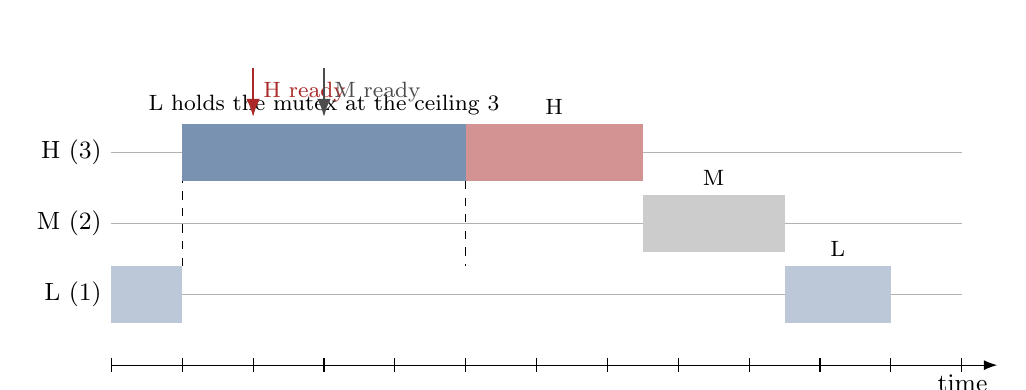
\begin{tikzpicture}[x=0.9cm,y=0.9cm,font=\small]
  % axes
  \draw[-{Latex}] (0,0) -- (12.5,0) node[below left] {time};
  \foreach \y/\n in {1/L (1),2/M (2),3/H (3)} {
    \draw[gray!60] (0,\y) -- (12,\y);
    \node[left] at (0,\y) {\n};
  }
  % L runs, locks at t=1 (raised to 3), unlocks at t=5
  \fill[nornblue!30] (0,0.6) rectangle (1,1.4);
  \fill[nornblue!60] (1,2.6) rectangle (5,3.4);
  \draw[dashed] (1,1.4) -- (1,2.6);
  \draw[dashed] (5,2.6) -- (5,1.4);
  \node[above,font=\footnotesize] at (3,3.4) {L holds the mutex at the ceiling 3};
  % H ready at t=2, runs at t=5
  \draw[-{Latex},nornred,thick] (2,4.2) -- (2,3.5) node[midway,right,font=\footnotesize] {H ready};
  \fill[nornred!50] (5,2.6) rectangle (7.5,3.4);
  \node[above,font=\footnotesize] at (6.25,3.4) {H};
  % M ready at t=3, runs after H
  \draw[-{Latex},black!70,thick] (3,4.2) -- (3,3.5) node[midway,right,font=\footnotesize] {M ready};
  \fill[gray!40] (7.5,1.6) rectangle (9.5,2.4);
  \node[above,font=\footnotesize] at (8.5,2.4) {M};
  \fill[nornblue!30] (9.5,0.6) rectangle (11,1.4);
  \node[above,font=\footnotesize] at (10.25,1.4) {L};
  \foreach \x in {0,1,...,12} \draw (\x,-0.1) -- (\x,0.1);
\end{tikzpicture}
\caption{Immediate priority ceiling. L (priority 1) locks a mutex with ceiling 3 at $t=1$
and runs at 3 until the unlock at $t=5$. H (3) and M (2) become ready meanwhile and
wait; H is delayed by one critical section of L and by nothing else, and M, which never
uses the mutex, is held off as long as L holds it. Nobody ever blocks on the mutex
itself.}
\label{fig:ceiling}
\end{figure}

\subsection{When the ceiling is wrong, or the owner blocks}

Two things break the ideal picture. A ceiling that is \emph{too low} (a task above the
ceiling locks the mutex) is a configuration error; the lock is asserted against it, and
without assertions the task finds the mutex held. And an owner may \emph{block while
holding} the mutex (allowed, discouraged): it then leaves the CPU at the ceiling, and a
task above its base priority but at or below the ceiling can run and try the lock.

For both cases the kernel has a fallback: the caller waits on the mutex, without a
timeout, and the unlock hands the mutex to the highest waiter, who becomes the owner at
the ceiling at once. A wait that would close a cycle of tasks waiting for each other's
mutexes is detected and is \code{RTOS\_PANIC\_DEADLOCK}, naming both tasks. The detector
follows chains of mutex waits only, which is why a task must not return while holding a
mutex (section~\ref{sec:lifecycle}): an owner that is gone would make every later lock
wait for ever without a cycle to detect.

\subsection{The order at equal effective priority}
\label{sec:tie}

While a task holds a mutex at the ceiling $c$, the task whose base priority is $c$ may
become ready. Both have effective priority $c$. The scheduling key from
section~\ref{sec:sched} settles it: the \emph{boosted} owner ranks above the task whose
base priority is the ceiling, so the owner finishes its critical section first and the
higher task does not preempt it. This is the choice that preserves the protocol's
promise that nobody blocks: were the task at the ceiling to preempt, it would find the
mutex locked. Two owners at one ceiling, which is possible only if one of them blocked
while holding, run in base priority order. The test \code{test/test\_tie.c} pins every
one of these cases down.

\subsection{Rules for using mutexes}

\begin{enumerate}
\item Set the ceiling to the highest priority of any task that locks the mutex, exactly.
\item Keep the critical section short; nothing below the ceiling runs meanwhile.
\item Do not block while holding a mutex. It is allowed, and the kernel copes, but it
  reintroduces waiting and it is the only way to get two tasks at one ceiling.
\item Lock in a fixed order and unlock in the reverse order (asserted). A mutex is not
  recursive (asserted).
\item Never return from a task function while holding a mutex (checked for every mutex
  whose ceiling is above the task's priority).
\item Do not lock from the idle task (asserted) or from an ISR body: an ISR body cannot
  wait, and a critical section is the right tool for a few instructions of shared state
  with an interrupt.
\end{enumerate}

\section{The task life cycle}
\label{sec:lifecycle}

A task slot is in one of five states, derived from the TCB rather than stored in it (no
state byte, no store on the hot path), with suspension as a modifier on top of READY and
BLOCKED:

\begin{table}[htbp]
\centering\small
\begin{tabularx}{\linewidth}{@{}lXll@{}}
\toprule
State & Predicate & Entered by & Left by \\
\midrule
UNUSED     & no task function; the TCB is in its initial state & \code{rtos\_init}, a future reap & \code{rtos\_createTask} \\
READY      & bit in the ready mask, not the running task & create, wake-up, preemption & pick, block, suspend \\
RUNNING    & the current task (its bit stays in the ready mask) & pick & block, preemption, return \\
BLOCKED    & bit not in the ready mask; \code{waitKind} says on what & a blocking call & wake-up, timeout \\
TERMINATED & \code{waitKind == RTOS\_WAIT\_TERMINATED} & the task function returning & a future reap \\
\bottomrule
\end{tabularx}
\caption{The task states. \code{rtos\_getTaskInfo} reports them as \code{RTOS\_TASK\_*},
with SUSPENDED for a suspended READY or BLOCKED task.}
\label{tab:states}
\end{table}

\begin{figure}[htbp]
\centering
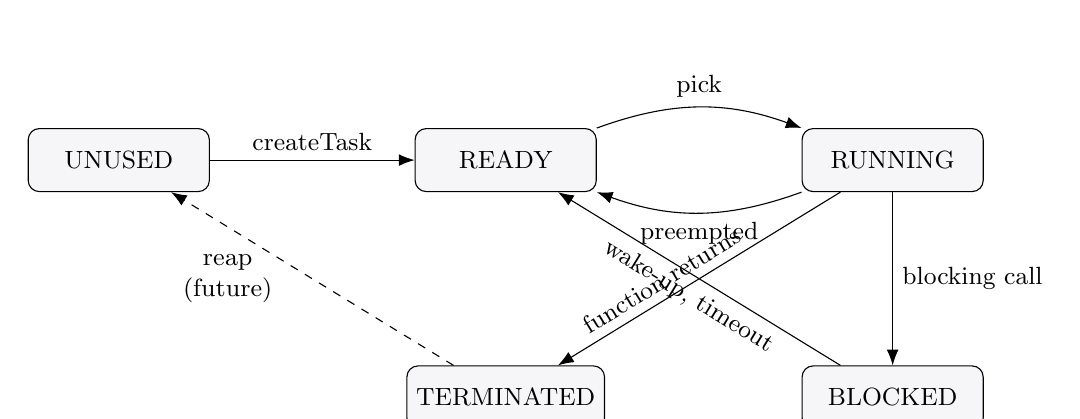
\begin{tikzpicture}[font=\small, node distance=2.2cm and 2.6cm,
  state/.style={draw, rounded corners, minimum width=2.3cm, minimum height=0.8cm, fill=codebg},
  >={Latex[length=2mm]}]
  \node[state] (unused) {UNUSED};
  \node[state, right=of unused] (ready) {READY};
  \node[state, right=of ready] (running) {RUNNING};
  \node[state, below=of running] (blocked) {BLOCKED};
  \node[state, below=of ready] (term) {TERMINATED};
  \draw[->] (unused) -- node[above] {createTask} (ready);
  \draw[->] (ready.north east) to[bend left=20] node[above] {pick} (running.north west);
  \draw[->] (running.south west) to[bend left=20] node[below] {preempted} (ready.south east);
  \draw[->] (running) -- node[right] {blocking call} (blocked);
  \draw[->] (blocked) -- node[below, sloped] {wake-up, timeout} (ready);
  \draw[->] (running) -- node[above, sloped, pos=0.6] {function returns} (term);
  \draw[->, dashed] (term) -- node[left, text width=1.9cm, align=center] {reap\\(future)} (unused);
\end{tikzpicture}
\caption{The life cycle of a task slot. Suspension (\code{rtos\_suspend}) is a modifier
on READY and BLOCKED, not a state: the task keeps its wait and its pending wake-ups and
continues at \code{rtos\_resume}.}
\label{fig:states}
\end{figure}

A task function \emph{should} never return. If it does, the task is terminated: its slot
and stack stay allocated, it is never scheduled again, and it is deaf to events,
notifications, suspends and resumes aimed at it (they accumulate or are ignored
harmlessly). Returning while holding a mutex is checked, for the reason given above. The
kernel does not yet reuse a terminated slot at run time; the rules under which a future
dynamic task API will do so are fixed (appendix~\ref{app:roadmap}), and the test
\code{test/test\_lifecycle.c} already verifies them against the kernel.

\section{Stacks}
\label{sec:stacks}

Each task runs on the stack given to \code{rtos\_createTask}. What a task needs is its
own frames plus what the kernel and the port leave under them when the task blocks or is
interrupted. An interrupt lands on the stack of the running task, so every task must
have room for the interrupt frame and the kernel's work on top of its own deepest call
chain. The port gives three sizes (table~\ref{tab:stacksizes}), and chapter~\ref{ch:perf}
has the measurements they are derived from.

\begin{table}[htbp]
\centering\small
\begin{tabularx}{\linewidth}{@{}lrrX@{}}
\toprule
Name & ESP32 & AVR & Meant for \\
\midrule
\code{RTOS\_STACK\_MIN}     & 512 B  & 96 B  & the technical minimum the kernel accepts (checked): very simple tasks whose use has been measured \\
\code{RTOS\_STACK\_DEFAULT} & 1024 B & 192 B & an ordinary task; start here \\
\code{RTOS\_STACK\_LARGE}   & 2048 B & 384 B & a recommended start for tasks that print, nest calls or use floating point; not an upper bound \\
\bottomrule
\end{tabularx}
\caption{The stack sizes the port names. Size a task from the default, run it, read the
high water mark with \code{rtos\_getStackFree}, and keep a margin above
\code{RTOS\_PORT\_STACK\_WARN} (96 B on the ESP32, 24 B on the AVR).}
\label{tab:stacksizes}
\end{table}

With \code{RTOS\_CFG\_STACK\_CHECK} the stack is filled with a pattern at creation and
the high water mark can be read; with \code{RTOS\_CFG\_STACK\_WARN} the idle task
watches one task per loop and calls \code{rtos\_stackWarnHook} once for a task whose
margin is gone; with \code{RTOS\_CFG\_STACK\_CHECK 2} a canary at the bottom turns an
actual overflow into \code{RTOS\_PANIC\_STACK\_OVERFLOW}, checked before every switch and
at every tick.

\chapter{Configuration}
\label{ch:config}

The kernel is configured at compile time by \code{rtos\_config.h} in the application
directory, started from \code{config/rtos\_config.template.h}. Every option has a
default (in \code{rtos\_types.h}) so a configuration lists only what differs, with one
exception: \code{RTOS\_CFG\_NUM\_TASKS} must be given.

\section{The options}

\begin{small}
\begin{longtable}{@{}lp{1.5cm}p{9.0cm}@{}}
\caption{The configuration options, all prefixed \code{RTOS\_CFG\_}.}
\label{tab:options}\\
\toprule
Option & Default & Meaning \\
\midrule
\endfirsthead
\toprule
Option & Default & Meaning \\
\midrule
\endhead
\bottomrule
\endlastfoot
\code{NUM\_TASKS}     & --      & application tasks, 1 to 31; the idle task is not counted; each gets the priority equal to its id \\
\code{TICK\_HZ}       & 1000    & tick frequency; on the AVR it must divide $F_{CPU}/64$ exactly (1000 and 500 work at 16 MHz) \\
\code{TICK\_BITS}     & 32      & width of the tick counter, 16 or 32; 16 saves RAM on the UNO and limits timeouts to 32.7 s \\
\code{EVT\_BITS}      & 16      & width of the per task event flags, 8, 16 or 32; nornWIFI needs 32 \\
\code{TIMER}          & arch    & AVR only: which 16 bit timer drives the tick (Mega: 1, 3, 4, 5; UNO: 1) \\
\code{STACK\_CHECK}   & 1       & 1 fills stacks and supports \code{rtos\_getStackFree}; 2 adds the canary; 0 drops the bookkeeping \\
\code{STACK\_WARN}    & 1       & the stack monitor in the idle task and \code{rtos\_stackWarnHook}; needs \code{STACK\_CHECK} \\
\code{IDLE\_SLEEP}    & 1       & the idle task sleeps between interrupts \\
\code{SW\_TIMERS}     & 1       & software timers; one list check per tick \\
\code{RUNTIME\_STATS} & 1       & run time per task and CPU load, measured at every switch; about 45 cycles per switch on the AVR, 4 bytes per task \\
\code{ASSERT}         & 1       & kernel assertions; about 20 cycles per switch on the AVR \\
\code{IDLE\_HOOK}     & --      & a function called in every idle loop; the weak \code{rtos\_idleHook} is the usual way \\
\code{PANIC\_ACTION}  & 0       & 0 halts at a panic (development), 1 resets with the record kept for \code{rtos\_getLastPanic} \\
\code{WATCHDOG}       & 0       & hardware watchdog kicked by the idle task plus per task check-ins \\
\code{AVR\_RESET\_VIA\_WDT} & 0 & AVR: reset through the watchdog (needs a bootloader that disables it) or by jumping to the reset vector \\
\code{TIMER\_TASK\_PRIO} & 0    & 0 runs timer callbacks in the tick interrupt; a priority runs them in a kernel task of that priority (\code{TIMER\_TASK\_STACK} sizes it) \\
\code{TRACE}          & 0       & call \code{rtos\_traceHook} at switches, blocks, wake-ups, timers and panics \\
\code{EVGROUPS}       & 1       & event groups \\
\code{NOTIFY}         & 1       & task notifications; 0 saves 2 bytes per task \\
\code{SUSPEND}        & 1       & \code{rtos\_suspend} and \code{rtos\_resume} \\
\code{HEAP}           & 0       & the first fit heap \\
\code{TICKLESS}       & 0       & ESP32: the idle task stops the tick and sleeps until the next deadline \\
\end{longtable}
\end{small}

\section{Three configurations to start from}

The three sets in table~\ref{tab:threecfg} are measured starting points. \emph{small} is
the lean kernel for the UNO or for the smallest possible footprint; \emph{default} is an
ordinary application, and what nornWIFI needs on the ESP32; \emph{large} turns on
everything for development and diagnosis.

\begin{table}[htbp]
\centering\small
\begin{tabular}{@{}llll@{}}
\toprule
Option & small & default & large \\
\midrule
\code{NUM\_TASKS} esp32 / mega / uno & 7 / 4 / 3 & 15 / 7 / 4 & 31 / 7 / -- \\
\code{TICK\_BITS} esp32 / avr        & 32 / 16   & 32 / 32 (uno 16) & 32 / 32 \\
\code{EVT\_BITS} esp32 / avr         & 16 / 8    & 32 / 16 (uno 8)  & 32 / 16 \\
\code{STACK\_CHECK}                  & 1         & 2 (canary)       & 2 \\
\code{STACK\_WARN}                   & 0         & 1                & 1 \\
\code{RUNTIME\_STATS}                & 0         & 1                & 1 \\
\code{ASSERT}                        & 0         & 1                & 1 \\
\code{EVGROUPS}, \code{SUSPEND}      & 0         & 1 (uno 0)        & 1 \\
\code{HEAP}, \code{WATCHDOG}         & 0         & esp32 1, avr 0   & esp32 1, avr 0 \\
\code{TRACE}                         & 0         & 0                & 1 \\
\code{TICKLESS} (esp32)              & 0         & 0                & 1 \\
\code{SW\_TIMERS}, \code{NOTIFY}     & 1 (uno: timers 0) & 1        & 1 \\
\midrule
switch, cycles, esp32 / mega         & 347 / 315 & 440 / 472        & 472 / -- \\
\bottomrule
\end{tabular}
\caption{Three configurations and their measured context switch (tc10, per switch
including the signalling). Common to all: \code{TICK\_HZ} 1000, \code{IDLE\_SLEEP} 1,
\code{TIMER\_TASK\_PRIO} 0, \code{PANIC\_ACTION} 0.}
\label{tab:threecfg}
\end{table}

Two constraints from the hardware: the original Mega 2560 bootloader does not survive a
watchdog reset, so the watchdog stays off on the AVR boards unless the bootloader is
replaced; and nornWIFI needs the heap, event groups and 32 event bits.

\section{The configuration signature}

\code{rtos\_init} is a macro that passes \code{RTOS\_CONFIG\_SIGNATURE}, every layout
changing option folded into one 32 bit number, to the kernel. An application compiled
against another \code{rtos\_config.h} than the kernel objects it is linked with (a stale
build directory, a library) panics with \code{RTOS\_PANIC\_CONFIG} at the first call,
before any TCB is touched; the record carries both signatures.

\section{A priority map}

Priorities are unique and the module tasks need to be above every task that uses them.
A map that works with the default configuration on the ESP32 (15 tasks): the nornWIFI
radio task at 15 and its service task at 14, the nornNET net task at 13, the
application's tasks from 1 to 12, with the most time critical highest. With the timer
task enabled (\code{TIMER\_TASK\_PRIO}) its slot must be left free by the application.
Period and deadline, not importance, should set the order among the application's
tasks: rate monotonic assignment is optimal for independent periodic tasks under fixed
priorities~\cite{liulayland}, and the ceiling protocol keeps the blocking term small
enough for the usual response time analysis~\cite{burnswellings} to apply.

\chapter{Using the primitives}
\label{ch:primitives}

nornCore offers more than one way to signal and to share. This chapter says what each
primitive is for, how it behaves at the edges, and shows the idiom. The formal contracts
are in chapter~\ref{ch:api}; the costs in chapter~\ref{ch:perf}.

\begin{table}[htbp]
\centering\small
\begin{tabularx}{\linewidth}{@{}lXl@{}}
\toprule
Need & Primitive & Cost, Mega / ESP32 \\
\midrule
wake one task, no data & task notification (\code{rtos\_notify}) or event flags & 220 / 145, 217 / 140 \\
count occurrences, producer to consumer & counting semaphore, or \code{RTOS\_NOTIFY\_INC} & 145 / 112 \\
hand a small record to another task, in order & message queue & 453 / 285 \\
the latest value only, overwrite is fine & mailbox & 282 / 194 \\
flags several tasks wait on & event group & 272 / 137 \\
protect shared data between tasks & ceiling mutex & 218 / 156 \\
fixed size buffers, bounded time & memory pool & 487 / 176 \\
variable size, rarely, at start-up & heap & -- \\
run something later or periodically without a task & software timer & 241 / 124 \\
\bottomrule
\end{tabularx}
\caption{Which primitive for which need. The costs are cycles for one call pair without a
switch (tc10, \measDate).}
\label{tab:which}
\end{table}

\section{Task event flags}

Every task owns \code{RTOS\_CFG\_EVT\_BITS} private event flags. Anyone posts
(\code{rtos\_postEvents}, \code{rtos\_postEventsFromIsr}, \code{rtos\_broadcastEvents}),
only the owner waits. Events posted earlier stay pending until a wait consumes them, so
nothing is lost between two waits; the wait returns the events that satisfied it and
clears those, leaving other pending events alone.

\begin{lstlisting}
#define EVT_SAMPLE  0x01u
#define EVT_BUTTON  0x02u

static void controller(void *arg)
{
    for(;;)
    {
        const rtos_evt_t got = rtos_waitEvents(EVT_SAMPLE | EVT_BUTTON, RTOS_WAIT_ANY, RTOS_MS(500));
        if(got == 0)            /* timeout: nothing in 500 ms */
            handleSilence();
        if(got & EVT_SAMPLE)
            processSample();
        if(got & EVT_BUTTON)
            handleButton();
    }
}

RTOS_ISR(ADC_vect)
{
    rtos_postEventsFromIsr(TASK_CONTROLLER, EVT_SAMPLE);
}
\end{lstlisting}

\code{RTOS\_WAIT\_ALL} waits for every bit of the mask. Event flags are the right tool
when one task is the hub of several sources; they carry no data and do not count.

\section{Counting semaphores}

A semaphore counts tokens. \code{rtos\_semGive} adds one, or hands it directly to the
highest waiting task; \code{rtos\_semTake} takes one or waits. \code{RTOS\_SEM\_INIT(n)}
makes a semaphore without an upper limit, \code{RTOS\_SEM\_INIT\_BINARY(n)} one whose
count never exceeds one (a give while the token is available is dropped and counted in
the \code{lost} field), \code{RTOS\_SEM\_INIT\_MAX(n, max)} one with any limit. The
typical use is an interrupt producing and a task consuming:

\begin{lstlisting}
static rtos_sem_t _rxReady = RTOS_SEM_INIT(0);

RTOS_ISR(USART0_RX_vect)
{
    _rxBuf[_rxIn++ & RX_MASK] = UDR0;
    rtos_semGiveFromIsr(&_rxReady);
}

static void reader(void *arg)
{
    for(;;)
        if(rtos_semTake(&_rxReady, RTOS_FOREVER))
            consume(_rxBuf[_rxOut++ & RX_MASK]);
}
\end{lstlisting}

The semaphore here is only the count; the data travels in the application's own ring. A
semaphore is not a lock: there is no owner and no priority ceiling, and using one for
mutual exclusion brings back the priority inversion the mutex exists to prevent.

\section{Ceiling mutexes}

A mutex protects shared data between tasks. Its one parameter is the ceiling, the highest
priority of any task that will lock it (section~\ref{sec:mutex}).

\begin{lstlisting}
#define TASK_LOG     1
#define TASK_SENSOR  2
#define TASK_CTRL    4

static rtos_mutex_t _stateLock = RTOS_MUTEX_INIT(TASK_CTRL);   /* highest user */
static struct state _state;

static void sensor(void *arg)        /* priority 2 */
{
    for(;;)
    {
        (void)rtos_waitPeriodic(RTOS_MS(10));
        const int16_t t = readTemperature();
        rtos_mutexLock(&_stateLock);     /* runs at 4 until the unlock */
        _state.temperature = t;
        rtos_mutexUnlock(&_stateLock);
    }
}
\end{lstlisting}

While the sensor task holds the lock it runs at priority 4, so the controller (4) cannot
preempt it and find the state half written, and the logger (1) is unaffected. The
critical section is a few stores; keep it that way. Do not call anything that may block
inside it.

\section{Message queues}

A queue is a FIFO of fixed size items copied by value, with blocking send and receive and
non-blocking \code{FromIsr} variants. A send to a queue with a blocked receiver copies
the item straight into the receiver's buffer. A full queue makes the sender wait or, with
\code{RTOS\_NO\_WAIT} or from an interrupt, fail; failed sends are counted in the
\code{dropped} field, and the high water mark in \code{maxCount}, so a queue sized too
small is visible.

\begin{lstlisting}
typedef struct { uint8_t channel; uint16_t value; } sample_t;

static uint8_t      _qStore[8 * sizeof(sample_t)];
static rtos_queue_t _q = RTOS_QUEUE_INIT(_qStore, sizeof(sample_t), 8);

RTOS_ISR(BOARD_APP_TIMER_VECT)
{
    sample_t s = { .channel = ADMUX & 0x0F, .value = ADC };
    (void)rtos_queueSendFromIsr(&_q, &s);        /* false if full: counted as dropped */
}

static void worker(void *arg)
{
    sample_t s;
    for(;;)
        if(rtos_queueReceive(&_q, &s, RTOS_MS(100)))
            process(&s);
        else
            noSampleFor100ms();
}
\end{lstlisting}

Items are copied twice (in and out), so a queue of large items is better replaced by a
queue of pointers into a memory pool.

\section{Mailboxes}

A mailbox is a queue of depth one in which a post never blocks and overwrites an unread
item (counted in \code{overwrites}). It carries \emph{the latest value}: a setpoint, a
measurement, a state that only the newest matters of. A reader blocks until something is
posted. Use it where a queue would only fill with stale data.

\section{Task notifications}

The cheapest signal: one 16 bit value per task and no object. \code{rtos\_notify}
replaces, ORs into or increments the value and wakes the task if it waits;
\code{rtos\_notifyWait} takes the whole value, \code{rtos\_notifyTake} waits for a
non-zero value and decrements it, which with \code{RTOS\_NOTIFY\_INC} on the sending side
is a counting semaphore without a semaphore. A task should use one of the two wait styles,
since they share the value. Notifications are the fastest switch on both boards
(figure~\ref{fig:switch}).

\begin{lstlisting}
RTOS_ISR(DMA_DONE_vect)
{
    rtos_notifyFromIsr(TASK_DMA, 1, RTOS_NOTIFY_INC);
}

static void dmaTask(void *arg)
{
    for(;;)
        if(rtos_notifyTake(RTOS_FOREVER))
            handleCompletion();
}
\end{lstlisting}

\section{Software timers}

A software timer calls a function after a delay, once or periodically, without a task of
its own. With \code{RTOS\_CFG\_TIMER\_TASK\_PRIO 0} the callback runs in the tick
interrupt with interrupts disabled: keep it short and use only the ISR body functions.
With a timer task configured, the callback runs in that task and may use the whole API,
at the price of a task slot and its stack.

\begin{lstlisting}
static rtos_timer_t _blink;

static void blinkCb(void *arg)
{
    gpio_toggle(&_led);                  /* ISR body: no blocking, no switch */
}

/* in a task or in main() before rtos_start: */
rtos_timerInit(&_blink, blinkCb, NULL);
rtos_timerStart(&_blink, RTOS_MS(500), RTOS_MS(500));   /* first in 500 ms, then every 500 ms */
\end{lstlisting}

The first expiry is on the \code{delay}-th tick from now (so after $\mathit{delay}-1$ to
$\mathit{delay}$ periods); later expiries are exactly \code{period} ticks apart, counted
from the previous expiry, so a periodic timer does not drift. A delay of 0 means the next
tick, which lets a callback restart its own timer. The active timers are a list sorted
by expiry; \code{rtos\_timerStart} spends time proportional to their number with
interrupts off.

\section{Memory pools}

A pool hands out fixed size blocks from storage the application owns, in constant time,
with a wait for a free block if wanted and a \code{FromIsr} variant that does not wait.
\code{rtos\_poolFree} checks that the block belongs to the pool and lies on a block
boundary. The low water mark \code{minFree} and the count of failed allocations
\code{failed} show whether the pool is sized right. A pool is what a driver uses for
packet buffers and what a queue of pointers refers to; it is the bounded time
alternative to the heap.

\begin{lstlisting}
static uint8_t     _frames[6 * 64];
static rtos_pool_t _framePool = RTOS_POOL_INIT(_frames, 64, 6);
/* rtos_poolInit(&_framePool, _frames, 64, 6) must still be called before use */

uint8_t *p = rtos_poolAlloc(&_framePool, RTOS_MS(10));
if(p != NULL) { fill(p); rtos_queueSend(&_frameQ, &p, RTOS_FOREVER); }
\end{lstlisting}

\section{Event groups}

An event group is a set of flags shared by any number of tasks
(\code{RTOS\_CFG\_EVGROUPS}). Where task event flags belong to one task, a group lets
several tasks wait for the same conditions: ``link up and address assigned'', say.
\code{rtos\_evgroupSet} wakes every waiter whose condition is now met, highest first; a
waiter that asked for \code{RTOS\_WAIT\_CLEAR} takes its bits out of the group as it is
woken, so a lower waiter no longer sees them. Without it the bits stay set for everyone
until \code{rtos\_evgroupClear}.

\section{Suspend and resume}

\code{rtos\_suspend} keeps a task from running until \code{rtos\_resume}, whatever it was
doing. A blocked task stays in its wait; a wake-up that arrives meanwhile is kept and
takes effect at the resume. There is no nesting count, and a suspended task keeps the
mutexes it holds, which is the reason to suspend only tasks that are known to hold none.
Suspension is for modes (``the display task is off while the lid is closed''), not for
synchronisation; the primitives above are.

\section{The heap}

\code{RTOS\_CFG\_HEAP} compiles a first fit allocator with coalescing over an area the
application gives it (\code{rtos\_heapInit}). \code{rtos\_malloc} searches the free list
with interrupts disabled, so its time grows with fragmentation; it is meant for
start-up allocations and for modules whose binary libraries need an allocator
(nornWIFI), not for the data path. \code{rtos\_heapStats} reports the low water mark and
the largest free block.

\chapter{Robustness and diagnostics}
\label{ch:robust}

A kernel for a device that runs unattended has to answer two questions: what does it do
when the application breaks a rule, and how does the engineer find out what happened. The
answers in nornCore are a small number of mandatory checks, a panic record that survives
a reset, and a set of diagnostics that read the kernel's own bookkeeping.

\section{Checks and assertions}

Every public function that takes a task id, a storage pointer, a stack size or a timeout
validates it with \code{RTOS\_CHECK}, in every configuration. A violation is a
\emph{panic} with \code{RTOS\_PANIC\_ARGUMENT} and the two offending values in the record;
there is no error return for an argument that would corrupt memory, because a return
value is what the caller that made the mistake would ignore. Contracts whose violation
costs more to detect than it is worth in a release build are \code{RTOS\_ASSERT}ed
instead and compiled only with \code{RTOS\_CFG\_ASSERT}: recursive locks, the unlock
order, a lock from the idle task, an empty event mask. Chapter~\ref{ch:api} marks every
entry \emph{checked} or \emph{asserted}.

\section{Panic and the record}

\code{rtos\_panic(reason, arg1, arg2)} disables interrupts, writes a record (reason,
running task, tick, the two arguments, and for an assertion the file and line) into
memory that survives a reset, calls \code{rtos\_panicHook} and then halts
(\code{RTOS\_CFG\_PANIC\_ACTION 0}) or resets the board (1). After a reset,
\code{rtos\_init} takes the record out of that memory and \code{rtos\_getLastPanic}
returns it once; \code{rtos\_getResetCause} says what the hardware thinks happened
(power on, external, brown out, watchdog, software).

\begin{table}[htbp]
\centering\small
\begin{tabularx}{\linewidth}{@{}lX@{}}
\toprule
Reason & Meaning, \code{arg1} / \code{arg2} \\
\midrule
\code{RTOS\_PANIC\_ASSERT}         & a failed \code{RTOS\_ASSERT}; file and line in the record \\
\code{RTOS\_PANIC\_STACK\_OVERFLOW} & the canary of task \code{arg1} was overwritten (\code{STACK\_CHECK 2}) \\
\code{RTOS\_PANIC\_WATCHDOG}       & task \code{arg1} did not check in; \code{RTOS\_NO\_TASK}: the idle task \\
\code{RTOS\_PANIC\_DEADLOCK}       & task \code{arg1} would wait for a mutex held, through a chain, by itself; \code{arg2} the owner \\
\code{RTOS\_PANIC\_FAULT}          & a CPU exception; cause and address from the port \\
\code{RTOS\_PANIC\_CONFIG}         & the application's and the kernel's configuration signatures differ \\
\code{RTOS\_PANIC\_ARGUMENT}       & a mandatory check refused an argument; the values \\
\code{RTOS\_PANIC\_APPLICATION}    & \code{rtos\_panic} called by the application; its own arguments \\
\bottomrule
\end{tabularx}
\caption{Panic reasons.}
\label{tab:panic}
\end{table}

tc05 provokes four of these in turn on the boards (an application panic, a stack
overflow, a late task, a starved idle task), lets each reset the board, and checks the
record after every reset.

\section{Stack checking}

Section~\ref{sec:stacks} has the sizes; this is the machinery. With
\code{RTOS\_CFG\_STACK\_CHECK} the stack is filled with a pattern at creation and
\code{rtos\_getStackFree} counts the untouched bytes from the bottom: the high water
mark since the start. With \code{RTOS\_CFG\_STACK\_WARN} the idle task reads one task's
mark per loop and calls \code{rtos\_stackWarnHook} once for a task whose margin drops
below \code{RTOS\_PORT\_STACK\_WARN}. With \code{STACK\_CHECK 2} a canary at the bottom
is checked before every context switch and at every tick, and an overwritten canary is
\code{RTOS\_PANIC\_STACK\_OVERFLOW}. The canary catches an overflow after the fact; the
monitor warns before it.

\section{The watchdog}

\code{RTOS\_CFG\_WATCHDOG} arms the hardware watchdog (\code{rtos\_wdtInit}) and lets the
idle task kick it, but only after checking that every monitored task
(\code{rtos\_wdtMonitor}) has called \code{rtos\_wdtCheckIn} within its interval. A late
task is \code{RTOS\_PANIC\_WATCHDOG} with a record; a starved idle task, which means a
runaway task or an interrupt storm, lets the hardware reset the board without one, and
the next boot sees \code{RTOS\_RESET\_WATCHDOG}. The two cases together cover both ways
a system can hang.

\section{Deadlock detection}

A mutex wait that would close a cycle (A waits for a mutex B holds while B waits for one
A holds, through any number of tasks) is detected at the moment of the wait and is
\code{RTOS\_PANIC\_DEADLOCK}. With correct ceilings a wait never happens, so the detector
is a safety net for a wrong ceiling or an owner that blocked while holding.

\section{Run time statistics and task information}

\code{RTOS\_CFG\_RUNTIME\_STATS} measures the time each task runs, at every switch, in
counts of \code{RTOS\_RUNTIME\_HZ}. \code{rtos\_getTaskRunTime} returns a task's total,
\code{rtos\_getCpuLoad} the share of time not spent in the idle task since the previous
call. \code{rtos\_getTaskInfo} is the snapshot for a console or a debugger: state,
priority and effective priority, what the task waits on and until when, stack size and
free, run time, overruns. \code{rtos\_getOverrunCount} reads and optionally resets a
periodic task's overruns. The kernel objects also carry their own statistics: lost gives
on a semaphore, dropped sends and the high water mark on a queue, overwrites on a mailbox,
failed allocations and the low water mark on a pool, the heap's statistics.

\section{Trace}

\code{RTOS\_CFG\_TRACE} calls \code{rtos\_traceHook(event, a, b)} at every context switch
(the tasks leaving and entering), every block (task and wait kind), every wake-up, every
timer expiry and every panic, with interrupts disabled. \code{hal/trace.h} is a ring
buffer recorder to override the hook with, and the host unit tests are built on exactly
this trace: each test compares the recorded sequence of (task, event, value) with the
expected one.

\chapter{API reference}
\label{ch:api}

The reference follows the groups of \code{kernel/rtos.h}. Every entry gives the
prototype, the behaviour, the parameters, the calling context, and which contracts are
\emph{checked} (always) or \emph{asserted} (\code{RTOS\_CFG\_ASSERT}). Unless an entry
says otherwise, a \code{timeout} is in ticks: \code{RTOS\_NO\_WAIT} polls,
\code{RTOS\_FOREVER} waits for good, any other value is at most
\code{RTOS\_MAX\_TIMEOUT} (checked). Functions that may wake a higher task run it before
they return; their \code{FromIsr} variants defer the switch to the end of the interrupt.
The generated reference (\code{make api} in nornDocs) has the same text per function
with the remaining details.

\clearpage
\section{Constants and types}

\begin{table}[htbp]
\centering\small
\begin{tabularx}{\linewidth}{@{}>{\raggedright\arraybackslash}p{0.38\linewidth}X@{}}
\toprule
Name & Meaning \\
\midrule
\code{RTOS\_VERSION}           & version string of the kernel \\
\code{RTOS\_IDLE\_TASK}        & 0, the idle task \\
\code{RTOS\_NUM\_TASKS}        & \code{RTOS\_CFG\_NUM\_TASKS + 1} \\
\code{RTOS\_NO\_TASK}          & 0xFF, ``no task'' \\
\code{RTOS\_STACK\_MIN / DEFAULT / LARGE} & the port's stack sizes (table~\ref{tab:stacksizes}) \\
\code{RTOS\_FOREVER}, \code{RTOS\_NO\_WAIT} & timeouts: never, poll \\
\code{RTOS\_MAX\_TIMEOUT}      & the longest finite timeout, half the tick range \\
\code{RTOS\_MS(ms)}            & milliseconds to ticks, at compile time \\
\code{RTOS\_WAIT\_ANY / ALL}   & options of \code{rtos\_waitEvents}, \code{rtos\_evgroupWait} \\
\code{RTOS\_WAIT\_CLEAR}       & \code{rtos\_evgroupWait}: take the satisfying bits out of the group \\
\code{RTOS\_NOTIFY\_SET / OR / INC} & operations of \code{rtos\_notify} \\
\code{RTOS\_SEM\_INIT(n)}, \code{RTOS\_SEM\_INIT\_BINARY(n)}, \code{RTOS\_SEM\_INIT\_MAX(n, max)} & static semaphore initialisers \\
\code{RTOS\_MUTEX\_INIT(ceiling)} & static mutex initialiser \\
\code{RTOS\_QUEUE\_INIT(storage, itemSize, capacity)} & static queue initialiser \\
\code{RTOS\_MBOX\_INIT(storage, itemSize)} & static mailbox initialiser \\
\code{RTOS\_POOL\_INIT(storage, blockSize, numBlocks)} & static pool initialiser; \code{rtos\_poolInit} is still required \\
\code{RTOS\_EVGROUP\_INIT(bits)} & static event group initialiser \\
\code{RTOS\_RUNTIME\_HZ}, \code{RTOS\_RUNTIME\_TO\_MS(t)} & run time counter frequency and conversion \\
\code{rtos\_tick\_t}, \code{rtos\_evt\_t}, \code{rtos\_taskmask\_t}, \code{rtos\_runtime\_t} & the tick, event flag, task mask and run time types; widths from the configuration and the port \\
\code{rtos\_taskFunc\_t}, \code{rtos\_timerFunc\_t} & \code{void f(void *arg)} \\
\code{rtos\_sem\_t}, \code{rtos\_mutex\_t}, \code{rtos\_queue\_t}, \code{rtos\_mbox\_t}, \code{rtos\_pool\_t}, \code{rtos\_timer\_t}, \code{rtos\_evgroup\_t} & the kernel objects; treat as opaque except for the statistics fields named in chapter~\ref{ch:robust} \\
\code{rtos\_taskInfo\_t}, \code{rtos\_panicInfo\_t}, \code{rtos\_heapStats\_t} & diagnostic records \\
\code{RTOS\_TASK\_*}, \code{RTOS\_WAIT\_*}, \code{RTOS\_RESET\_*}, \code{RTOS\_TRACE\_*} & task states, wait kinds, reset causes, trace events \\
\bottomrule
\end{tabularx}
\caption{Constants and types.}
\end{table}

% -----------------------------------------------------------------------------------------
\section{Kernel life cycle}

\apihead{rtos\_init}
\begin{lstlisting}
#define rtos_init()   rtos_initChecked(RTOS_CONFIG_SIGNATURE)
\end{lstlisting}
Resets all kernel data: every task slot, the ready mask, the wake-up list and the tick
count, and takes the panic record of the previous boot out of the memory that survives a
reset. The macro passes the configuration signature; a kernel compiled with another
configuration stops at once with \code{RTOS\_PANIC\_CONFIG}.
\apipre{Called from \code{main()}, before any other kernel function, once.}

\apihead{rtos\_createTask}
\begin{lstlisting}
void rtos_createTask(uint8_t prio, rtos_taskFunc_t taskFunc, void *arg,
                     uint8_t *stackArea, size_t stackSize);
\end{lstlisting}
Creates the task at priority \code{prio} on the caller's stack. The task is ready at once
and runs at the earliest at \code{rtos\_start}. The stack start is aligned up and the
size rounded down to the port's alignment (1 byte on the AVR, 16 on the ESP32), which
may reduce the usable size; with \code{RTOS\_CFG\_STACK\_CHECK} the area is filled with
the pattern.
\begin{apiparams}
\item[prio] task priority and id, 1 to \code{RTOS\_CFG\_NUM\_TASKS}; the slot must be free.
\item[taskFunc] the task's function; should never return (section~\ref{sec:lifecycle}).
\item[arg] passed to the function unchanged.
\item[stackArea, stackSize] caller allocated memory, valid for as long as the system
  runs; at least \code{RTOS\_STACK\_MIN} after alignment.
\end{apiparams}
\apipre{After \code{rtos\_init}, before \code{rtos\_start}. Creating a task while the
scheduler runs is not supported yet.}
\apichecked{\code{prio} out of range, a NULL function or stack, a slot in use, a stack
below the minimum.}

\apihead{rtos\_start}
\begin{lstlisting}
void rtos_start(void);
\end{lstlisting}
Creates the timer task if configured, starts the tick, switches to the highest ready
task and never returns. The calling context becomes the idle task.

% -----------------------------------------------------------------------------------------
\section{Time and delays}

\apihead{rtos\_getTick}
\begin{lstlisting}
rtos_tick_t rtos_getTick(void);
\end{lstlisting}
\apireturns{the ticks since \code{rtos\_start}. The counter wraps (16 bits: 65.5 s at
1 kHz; 32 bits: 49.7 days); compare as differences.}
\apicontext{any.}

\apihead{rtos\_delay}
\begin{lstlisting}
void rtos_delay(rtos_tick_t ticks);
\end{lstlisting}
Blocks the calling task for at least \code{ticks} ticks; the real delay is between
\code{ticks} and \code{ticks + 1} periods. A delay of 0 waits for the next tick. Any
value is accepted: a delay above \code{RTOS\_MAX\_TIMEOUT} is done as a sequence of
waits, \code{RTOS\_FOREVER} blocks for good.
\apicontext{task; not the idle task (checked).}

\apihead{rtos\_waitPeriodic}
\begin{lstlisting}
bool rtos_waitPeriodic(rtos_tick_t period);
\end{lstlisting}
Blocks until the task's next period boundary; each boundary is the previous one plus
\code{period}, so the task runs drift free. If the boundary has passed, the call returns
at once, counts an overrun and computes the next boundary from now. The first boundary
is the task's start plus \code{period}. The period may change from call to call.
\begin{apiparams}
\item[period] 1 to \code{RTOS\_MAX\_TIMEOUT}.
\end{apiparams}
\apireturns{\code{true} on an overrun, \code{false} after a normal wait.}
\apicontext{task; not the idle task.}
\apichecked{a period of 0 or above the limit.}

% -----------------------------------------------------------------------------------------
\section{Task event flags}

\apihead{rtos\_waitEvents}
\begin{lstlisting}
rtos_evt_t rtos_waitEvents(rtos_evt_t mask, uint8_t opt, rtos_tick_t timeout);
\end{lstlisting}
Waits until events of \code{mask} are pending for the calling task. Events posted
earlier stay pending until a wait consumes them. The events that satisfy the wait are
cleared and returned; pending events outside the mask are kept.
\begin{apiparams}
\item[mask] the events to wait for; not 0 (asserted).
\item[opt] \code{RTOS\_WAIT\_ANY} or \code{RTOS\_WAIT\_ALL}.
\end{apiparams}
\apireturns{the consumed events (with \code{RTOS\_WAIT\_ALL}: the mask); 0 on timeout.}
\apicontext{task; the idle task may only poll.}

\apihead{rtos\_postEvents, rtos\_postEventsFromIsr}
\begin{lstlisting}
void rtos_postEvents(uint8_t taskId, rtos_evt_t events);
void rtos_postEventsFromIsr(uint8_t taskId, rtos_evt_t events);
\end{lstlisting}
ORs the events into the task's pending events; a task whose wait is thereby satisfied
becomes ready.
\apichecked{\code{taskId} 1 to \code{RTOS\_CFG\_NUM\_TASKS}.}

\apihead{rtos\_broadcastEvents}
\begin{lstlisting}
void rtos_broadcastEvents(rtos_evt_t events);
\end{lstlisting}
Posts the events to every created task (not the idle task).
\apicontext{task.}

% -----------------------------------------------------------------------------------------
\section{Counting semaphores}

\apihead{rtos\_semInit, rtos\_semInitMax}
\begin{lstlisting}
void rtos_semInit(rtos_sem_t *pSem, uint8_t initialCount);
void rtos_semInitMax(rtos_sem_t *pSem, uint8_t initialCount, uint8_t maxCount);
\end{lstlisting}
The run time alternatives to the static initialisers. Without a limit the count is
bounded by its type, 255; with \code{maxCount} a give at the limit is dropped and counted
as lost (1 makes a binary semaphore).
\apipre{no task waits on the semaphore.}
\apiasserted{\code{initialCount} at most \code{maxCount}, \code{maxCount} at least 1.}

\apihead{rtos\_semTake}
\begin{lstlisting}
bool rtos_semTake(rtos_sem_t *pSem, rtos_tick_t timeout);
\end{lstlisting}
Takes one token, waiting up to \code{timeout} for it.
\apireturns{\code{true} if a token was taken, \code{false} on timeout.}
\apicontext{task; the idle task may only poll.}

\apihead{rtos\_semGive, rtos\_semGiveFromIsr}
\begin{lstlisting}
void rtos_semGive(rtos_sem_t *pSem);
void rtos_semGiveFromIsr(rtos_sem_t *pSem);
\end{lstlisting}
Gives one token. If tasks wait, the highest gets it directly and the count does not
change; otherwise the count goes up or, at the limit, the give is lost.

% -----------------------------------------------------------------------------------------
\section{Ceiling mutexes}

\apihead{rtos\_mutexInit}
\begin{lstlisting}
void rtos_mutexInit(rtos_mutex_t *pMutex, uint8_t ceilingPrio);
\end{lstlisting}
The run time alternative to \code{RTOS\_MUTEX\_INIT}. \code{ceilingPrio} is the highest
priority of any task that will ever lock the mutex.
\apipre{the mutex is not locked.}

\apihead{rtos\_mutexLock}
\begin{lstlisting}
void rtos_mutexLock(rtos_mutex_t *pMutex);
\end{lstlisting}
Raises the caller's effective priority to the ceiling and takes the mutex. With a correct
ceiling the call never blocks. If the mutex is held anyway (a ceiling too low, or an
owner that blocked while holding), the caller waits without a timeout and the unlock
hands the mutex over to the highest waiter.
\apicontext{task; not the idle task (asserted).}
\apiasserted{the caller does not already hold the mutex (not recursive); the caller's
priority is at most the ceiling.}
\apinote{Panics}{a wait that would close a cycle of mutex waits is
\code{RTOS\_PANIC\_DEADLOCK} (the caller, the owner).}

\apihead{rtos\_mutexUnlock}
\begin{lstlisting}
void rtos_mutexUnlock(rtos_mutex_t *pMutex);
\end{lstlisting}
Drops the caller's effective priority back to what it was before the lock. A waiting
task becomes the owner at once, at the ceiling. Either change may let another task run
before the call returns.
\apicontext{task.}
\apiasserted{the caller owns the mutex; mutexes are unlocked in the reverse order of
locking.}

% -----------------------------------------------------------------------------------------
\section{Message queues}

\apihead{rtos\_queueInit}
\begin{lstlisting}
void rtos_queueInit(rtos_queue_t *pQ, uint8_t *storage, uint8_t itemSize, uint8_t capacity);
\end{lstlisting}
The run time alternative to \code{RTOS\_QUEUE\_INIT}. \code{storage} holds
\code{itemSize * capacity} bytes and stays valid for as long as the queue is used.
\apichecked{a NULL storage, an item size or a capacity of 0.}

\apihead{rtos\_queueSend, rtos\_queueSendFromIsr}
\begin{lstlisting}
bool rtos_queueSend(rtos_queue_t *pQ, const void *pItem, rtos_tick_t timeout);
bool rtos_queueSendFromIsr(rtos_queue_t *pQ, const void *pItem);
\end{lstlisting}
Copies an item into the queue, waiting up to \code{timeout} for room (the ISR variant
never waits). If a task is blocked in receive, the item goes straight into that task's
buffer. While the caller waits, the item is read at the moment a receiver frees a slot:
it must not change until the call returns. A failed send is counted as dropped.
\apireturns{\code{true} if the item was queued.}

\apihead{rtos\_queueReceive, rtos\_queueReceiveFromIsr}
\begin{lstlisting}
bool rtos_queueReceive(rtos_queue_t *pQ, void *pItem, rtos_tick_t timeout);
bool rtos_queueReceiveFromIsr(rtos_queue_t *pQ, void *pItem);
\end{lstlisting}
Copies the oldest item out, waiting up to \code{timeout} for one. If a sender is blocked
because the queue was full, its item moves into the freed slot.
\apireturns{\code{true} if an item was received.}

\apihead{rtos\_queueCount}
\begin{lstlisting}
uint8_t rtos_queueCount(const rtos_queue_t *pQ);
\end{lstlisting}
\apireturns{the items stored now; a snapshot.} \apicontext{any.}

% -----------------------------------------------------------------------------------------
\section{Mailboxes}

\apihead{rtos\_mboxInit, rtos\_mboxPost, rtos\_mboxPostFromIsr, rtos\_mboxFetch, rtos\_mboxIsFull}
\begin{lstlisting}
void rtos_mboxInit(rtos_mbox_t *pMb, uint8_t *storage, uint8_t itemSize);
bool rtos_mboxPost(rtos_mbox_t *pMb, const void *pItem);
bool rtos_mboxPostFromIsr(rtos_mbox_t *pMb, const void *pItem);
bool rtos_mboxFetch(rtos_mbox_t *pMb, void *pItem, rtos_tick_t timeout);
bool rtos_mboxIsFull(const rtos_mbox_t *pMb);
\end{lstlisting}
A post never blocks: it replaces an unread item (counted in \code{overwrites}, and the
post returns \code{true}) or, if a task is blocked in fetch, copies the item straight
into that task's buffer. A fetch takes the item and leaves the mailbox empty; it returns
\code{false} on timeout. \code{rtos\_mboxIsFull} tells whether an unread item waits.
\apichecked{\code{rtos\_mboxInit}: a NULL storage or an item size of 0.}

% -----------------------------------------------------------------------------------------
\section{Task notifications}

\apihead{rtos\_notify, rtos\_notifyFromIsr}
\begin{lstlisting}
void rtos_notify(uint8_t taskId, uint16_t value, uint8_t op);
void rtos_notifyFromIsr(uint8_t taskId, uint16_t value, uint8_t op);
\end{lstlisting}
Updates the task's 16 bit notification value and wakes the task if it waits in
\code{rtos\_notifyWait}, or in \code{rtos\_notifyTake} and the value is now non-zero.
\begin{apiparams}
\item[op] \code{RTOS\_NOTIFY\_SET} replaces the value, \code{RTOS\_NOTIFY\_OR} ORs
  \code{value} in, \code{RTOS\_NOTIFY\_INC} adds one, saturating at 0xFFFF.
\end{apiparams}
\apichecked{\code{taskId}.}

\apihead{rtos\_notifyWait}
\begin{lstlisting}
bool rtos_notifyWait(uint16_t *pValue, rtos_tick_t timeout);
\end{lstlisting}
Returns as soon as any notification has arrived since the last successful wait, even one
that set the value to 0, stores the value in \code{*pValue} (may be NULL) and resets it to 0.
\apicontext{task; the idle task may only poll.}

\apihead{rtos\_notifyTake}
\begin{lstlisting}
bool rtos_notifyTake(rtos_tick_t timeout);
\end{lstlisting}
Waits until the value is non-zero and decrements it by one: with
\code{RTOS\_NOTIFY\_INC} on the sending side, a counting semaphore without an object. A
task should use either \code{rtos\_notifyWait} or \code{rtos\_notifyTake}, not both.

% -----------------------------------------------------------------------------------------
\section{Software timers}

\apihead{rtos\_timerInit}
\begin{lstlisting}
void rtos_timerInit(rtos_timer_t *pT, rtos_timerFunc_t callback, void *arg);
\end{lstlisting}
Prepares an inactive timer. Where the callback runs depends on
\code{RTOS\_CFG\_TIMER\_TASK\_PRIO}: in the tick interrupt (0; only ISR body functions
allowed) or in the timer task.
\apichecked{a NULL callback.}

\apihead{rtos\_timerStart}
\begin{lstlisting}
void rtos_timerStart(rtos_timer_t *pT, rtos_tick_t delay, rtos_tick_t period);
\end{lstlisting}
Arms the timer, or restarts it if active. The first expiry is on the \code{delay}-th tick
from now (after \code{delay - 1} to \code{delay} periods; 0 and 1 both mean the next
tick); after that every \code{period} ticks exactly, counted from the previous expiry.
\code{period} 0 is a one shot timer. The time spent with interrupts disabled grows with
the number of active timers.
\apicontext{any.}
\apichecked{the timer was initialised; \code{delay} and \code{period} at most the limit.}

\apihead{rtos\_timerStop, rtos\_timerIsActive, rtos\_timerRemaining}
\begin{lstlisting}
void        rtos_timerStop(rtos_timer_t *pT);
bool        rtos_timerIsActive(const rtos_timer_t *pT);
rtos_tick_t rtos_timerRemaining(const rtos_timer_t *pT);
\end{lstlisting}
Disarms the timer (nothing happens if it is not active; with a timer task an expiry
still waiting for the task is dropped, a running callback finishes); tells whether it is
armed; returns the ticks to the next expiry (0 if inactive or due).
\apicontext{any.}

% -----------------------------------------------------------------------------------------
\section{Memory pools}

\apihead{rtos\_poolInit}
\begin{lstlisting}
void rtos_poolInit(rtos_pool_t *pPool, uint8_t *storage, uint16_t blockSize, uint8_t numBlocks);
\end{lstlisting}
Builds the free list over the storage; also required after \code{RTOS\_POOL\_INIT}. A
block is returned at the alignment of its offset in the storage, so storage meant for
aligned objects must be aligned itself and have a block size that is a multiple of that
alignment.
\apichecked{a NULL storage, a block size below \code{sizeof(void *)}, 0 blocks.}

\apihead{rtos\_poolAlloc, rtos\_poolAllocFromIsr}
\begin{lstlisting}
void *rtos_poolAlloc(rtos_pool_t *pPool, rtos_tick_t timeout);
void *rtos_poolAllocFromIsr(rtos_pool_t *pPool);
\end{lstlisting}
Gets a block, waiting up to \code{timeout} for one to be freed (the ISR variant never
waits). A failed allocation is counted.
\apireturns{the block, or NULL.}

\apihead{rtos\_poolFree, rtos\_poolFreeFromIsr, rtos\_poolFreeCount}
\begin{lstlisting}
void    rtos_poolFree(rtos_pool_t *pPool, void *pBlock);
void    rtos_poolFreeFromIsr(rtos_pool_t *pPool, void *pBlock);
uint8_t rtos_poolFreeCount(const rtos_pool_t *pPool);
\end{lstlisting}
Returns a block; a task waiting for one gets it directly.
\apichecked{a pointer outside the pool or not at the start of a block. A double free is
caught only when the pool would hold more free blocks than it has.}

% -----------------------------------------------------------------------------------------
\section{Event groups}

\apihead{rtos\_evgroupInit, rtos\_evgroupSet, rtos\_evgroupSetFromIsr, rtos\_evgroupClear, rtos\_evgroupGet}
\begin{lstlisting}
void       rtos_evgroupInit(rtos_evgroup_t *pG, rtos_evt_t initialBits);
void       rtos_evgroupSet(rtos_evgroup_t *pG, rtos_evt_t bits);
void       rtos_evgroupSetFromIsr(rtos_evgroup_t *pG, rtos_evt_t bits);
void       rtos_evgroupClear(rtos_evgroup_t *pG, rtos_evt_t bits);
rtos_evt_t rtos_evgroupGet(const rtos_evgroup_t *pG);
\end{lstlisting}
Set wakes every waiter whose condition is now met, highest priority first; a waiter that
asked for \code{RTOS\_WAIT\_CLEAR} takes its bits out as it is woken. Clear wakes nobody.
With waiters present, set checks every task slot with interrupts disabled.

\apihead{rtos\_evgroupWait}
\begin{lstlisting}
rtos_evt_t rtos_evgroupWait(rtos_evgroup_t *pG, rtos_evt_t mask, uint8_t options,
                            rtos_tick_t timeout);
\end{lstlisting}
Waits until bits of \code{mask} are set. \code{options} is \code{RTOS\_WAIT\_ANY} or
\code{RTOS\_WAIT\_ALL}, optionally with \code{RTOS\_WAIT\_CLEAR}.
\apireturns{the satisfying bits (with ALL: the mask); 0 on timeout.}
\apiasserted{\code{mask} not 0.}

% -----------------------------------------------------------------------------------------
\section{Suspend and resume}

\apihead{rtos\_suspend, rtos\_resume, rtos\_resumeFromIsr}
\begin{lstlisting}
void rtos_suspend(uint8_t taskId);
void rtos_resume(uint8_t taskId);
void rtos_resumeFromIsr(uint8_t taskId);
\end{lstlisting}
Suspend keeps the task from running until a resume; a blocked task stays in its wait, a
wake-up that arrives meanwhile takes effect at the resume. No nesting count; a task may
suspend itself. A suspended task keeps its mutexes. Resume does nothing to a task that is
not suspended.
\apichecked{\code{taskId}; not the idle task.}

% -----------------------------------------------------------------------------------------
\section{Heap}

\apihead{rtos\_heapInit, rtos\_malloc, rtos\_free, rtos\_heapStats}
\begin{lstlisting}
void  rtos_heapInit(void *area, size_t size);
void *rtos_malloc(size_t size);
void  rtos_free(void *p);
void  rtos_heapStats(rtos_heapStats_t *pStats);
\end{lstlisting}
A first fit allocator with coalescing over the area given once to \code{rtos\_heapInit}.
Blocks are aligned to \code{2 * sizeof(void *)}. The search runs with interrupts
disabled and its time grows with the number of free blocks. \code{rtos\_free} ignores
NULL.
\apicontext{task.}
\apichecked{a NULL or too small area; \code{rtos\_malloc} before \code{rtos\_heapInit};
a freed pointer outside the heap or already free. A pointer into the middle of a block is
not detected.}

% -----------------------------------------------------------------------------------------
\section{Diagnostics}

\apihead{rtos\_getCurrentTask}
\begin{lstlisting}
uint8_t rtos_getCurrentTask(void);
\end{lstlisting}
\apireturns{the running task's id; 0 in the idle task; in an ISR body the interrupted task.}

\apihead{rtos\_getOverrunCount}
\begin{lstlisting}
uint8_t rtos_getOverrunCount(uint8_t taskId, bool reset);
\end{lstlisting}
\apireturns{the period overruns of the task since the start or the last reset; saturates
at 255. \code{reset} clears the counter after reading.} \apichecked{\code{taskId} 0 to
\code{RTOS\_CFG\_NUM\_TASKS}.}

\apihead{rtos\_getStackFree}
\begin{lstlisting}
size_t rtos_getStackFree(uint8_t taskId);
\end{lstlisting}
\apireturns{the bytes at the bottom of the task's stack never used since creation; 0 for
the idle task, a task never created, or without \code{RTOS\_CFG\_STACK\_CHECK}. The scan
reads the stack byte by byte with interrupts enabled.}

\apihead{rtos\_getTimeUs}
\begin{lstlisting}
uint32_t rtos_getTimeUs(void);
\end{lstlisting}
\apireturns{microseconds since start from the port's free running time base; wraps after
71.6 minutes.} \apicontext{any.}

\apihead{rtos\_getTaskRunTime, rtos\_getCpuLoad}
\begin{lstlisting}
rtos_runtime_t rtos_getTaskRunTime(uint8_t taskId);
uint8_t        rtos_getCpuLoad(void);
\end{lstlisting}
With \code{RTOS\_CFG\_RUNTIME\_STATS}: the accumulated run time of a task in counts of
\code{RTOS\_RUNTIME\_HZ} (the running task's includes the current slice), and the share
of time not spent in the idle task since the previous call, 0 to 100. Every call of
\code{rtos\_getCpuLoad} starts a new interval, so one task should own the readings.

\apihead{rtos\_getTaskInfo}
\begin{lstlisting}
bool rtos_getTaskInfo(uint8_t taskId, rtos_taskInfo_t *pInfo);
\end{lstlisting}
Fills a snapshot: state (\code{RTOS\_TASK\_*}), priority, effective priority, wait kind
and object, timeout, stack size and free, run time, overruns.
\apireturns{\code{true}; \code{false} for an id out of range or a NULL \code{pInfo}
(not a panic).}

% -----------------------------------------------------------------------------------------
\section{Panic and reset cause}

\apihead{rtos\_panic}
\begin{lstlisting}
void rtos_panic(uint8_t reason, uint32_t arg1, uint32_t arg2) __attribute__((noreturn));
\end{lstlisting}
Disables interrupts, records the reason and the arguments in memory that survives a
reset, calls \code{rtos\_panicHook} and halts or resets (\code{RTOS\_CFG\_PANIC\_ACTION}).
Applications use \code{RTOS\_PANIC\_APPLICATION}.
\apicontext{any.}

\apihead{rtos\_getLastPanic, rtos\_getResetCause}
\begin{lstlisting}
bool    rtos_getLastPanic(rtos_panicInfo_t *pInfo);
uint8_t rtos_getResetCause(void);
\end{lstlisting}
The record left before the last reset, reported in one boot only (\code{pInfo} may be
NULL to ask only), and the cause of the last reset as the hardware reports it
(\code{RTOS\_RESET\_*}).

% -----------------------------------------------------------------------------------------
\section{Hooks}

\apihead{rtos\_idleHook, rtos\_panicHook, rtos\_stackWarnHook, rtos\_assertFailed, rtos\_traceHook}
\begin{lstlisting}
void rtos_idleHook(void);
void rtos_panicHook(const rtos_panicInfo_t *pInfo);
void rtos_stackWarnHook(uint8_t task, size_t stackFree);
void rtos_assertFailed(const char *file, uint16_t line) __attribute__((noreturn, cold));
void rtos_traceHook(uint8_t event, uint32_t a, uint32_t b);
\end{lstlisting}
Weak functions the application overrides. The idle hook runs in every idle loop and
must not block. The panic hook runs with interrupts disabled before the halt or reset and
must not call the kernel. The stack warning hook is called once per task whose margin is
gone. \code{rtos\_assertFailed} is called for a failed assertion; its default stores file
and line and panics, and an override must not return either. The trace hook is called
with interrupts disabled at every traced event (\code{RTOS\_TRACE\_SWITCH}, \code{BLOCK},
\code{READY}, \code{TIMER}, \code{PANIC}) and must not call the kernel.

% -----------------------------------------------------------------------------------------
\section{Watchdog}

\apihead{rtos\_wdtInit, rtos\_wdtMonitor, rtos\_wdtCheckIn}
\begin{lstlisting}
void rtos_wdtInit(uint32_t timeoutMs);
void rtos_wdtMonitor(uint8_t task, rtos_tick_t maxInterval);
void rtos_wdtCheckIn(void);
\end{lstlisting}
Starts the hardware watchdog (the timeout is rounded up to what the hardware offers;
the idle task kicks it only after \code{rtos\_start}); requires a task to check in at
least every \code{maxInterval} ticks (0 stops monitoring it; the first deadline is
\code{maxInterval} from now); tells the watchdog the calling task is alive.
\apichecked{\code{task}; \code{maxInterval} at most the limit.}
\apiasserted{\code{timeoutMs} above 0.}

\chapter{Networking: nornNET, nornWIFI and nornHTTP}
\label{ch:net}

The network modules are separate repositories with their own READMEs and plans; this
chapter is what an application writer needs to use them from nornRTOS. The design
sketch, protocol scope and test record are in \code{nornNET/doc/plan.md},
\code{nornWIFI/doc/plan.md} and \code{nornHTTP/docs/} (contracts, measurements, plan).

\section{nornNET}

nornNET is a small TCP/IP stack: Ethernet, ARP, IPv4, ICMP, UDP, TCP (RFC 9293 with slow
start, fast retransmit, delayed ACK, Nagle, zero window probing and out of order
storage), a DHCP client and a DNS resolver, loosely modelled on microps~\cite{microps} in
structure. Packet buffers are fixed size blocks from a pool, owned by whoever holds the
pointer; there is one net task, one re-entrant lock, and no heap in the data path. It is
verified against the Linux kernel as the peer, over a TAP device, QEMU's user mode
network and a serial line (SLIP) on the ESP32 board, and it runs on the Mega 2560 over
SLIP at the line rate.

\subsection{Attaching it to an application}

In \code{app.mk}:
\begin{lstlisting}[language={}]
NORNNET_DIR = /path/to/nornNET
MODULES    += $(NORNNET_DIR)/nornnet.mk
\end{lstlisting}
and an \code{nn\_config.h} next to the application with at least
\code{NN\_CFG\_TASK\_PRIO}, the net task's priority, above every task that uses the
stack. Every \code{NN\_CFG\_*} option and its default is in \code{nn/nn\_cfg.h}. In
\code{main}, after \code{rtos\_init}: \code{nn\_init()}, register the devices, add the
interfaces with \code{nn\_ifaceAdd} (with an address, or empty and \code{nn\_dhcpStart}
from a task), then \code{rtos\_start()}.

\subsection{Sockets}

Sockets are caller owned objects; for TCP the caller also owns the send and receive
rings. Each call is either blocking with a timeout, from a task, or a callback that runs
in the net task. The lock is re-entrant for the net task, so a callback may call the
socket API.

\begin{lstlisting}
nn_err_t nn_udpOpen(nn_udp_t *pSock);
nn_err_t nn_udpBind(nn_udp_t *pSock, nn_ip4_t addr, uint16_t port);
nn_err_t nn_udpConnect(nn_udp_t *pSock, nn_ip4_t addr, uint16_t port);
nn_err_t nn_udpSendTo(nn_udp_t *pSock, const void *p, size_t n, nn_ip4_t to, uint16_t port);
nn_err_t nn_udpSend(nn_udp_t *pSock, const void *p, size_t n);
int32_t  nn_udpRecvFrom(nn_udp_t *pSock, void *p, size_t n, nn_ip4_t *pFrom,
                        uint16_t *pPort, nn_ms_t timeout);
void     nn_udpOnReadable(nn_udp_t *pSock, nn_udpReadableFunc_t fn, void *arg);
nn_err_t nn_udpClose(nn_udp_t *pSock);

nn_err_t nn_tcpOpen(nn_tcp_t *pSock, void *pRxRing, uint16_t rxSize, void *pTxRing, uint16_t txSize);
nn_err_t nn_tcpBind(nn_tcp_t *pSock, nn_ip4_t addr, uint16_t port);
nn_err_t nn_tcpListen(nn_tcp_t *pSock);
nn_err_t nn_tcpAccept(nn_tcp_t *pListen, nn_tcp_t *pNew, nn_ms_t timeout);
nn_err_t nn_tcpConnect(nn_tcp_t *pSock, nn_ip4_t addr, uint16_t port, nn_ms_t timeout);
int32_t  nn_tcpSend(nn_tcp_t *pSock, const void *p, size_t n, nn_ms_t timeout);
int32_t  nn_tcpRecv(nn_tcp_t *pSock, void *p, size_t n, nn_ms_t timeout);
nn_err_t nn_tcpClose(nn_tcp_t *pSock);
nn_err_t nn_tcpAbort(nn_tcp_t *pSock);
void     nn_tcpOnEvent(nn_tcp_t *pSock, nn_tcpEventFunc_t fn, void *arg);

nn_err_t nn_dhcpStart(nn_dhcp_t *pD, nn_iface_t *pIf, nn_dhcpChangeFunc_t fn, void *arg);
nn_err_t nn_dnsResolve(const char *name, nn_ip4_t *pAddr, nn_ms_t timeout);
\end{lstlisting}

Errors are negative \code{nn\_err\_t} values: \code{NN\_ERR\_NOMEM} (no buffer),
\code{NN\_ERR\_TIMEOUT}, \code{NN\_ERR\_DOWN} (the device or the address is gone),
\code{NN\_ERR\_RESET}, \code{NN\_ERR\_REFUSED}, \code{NN\_ERR\_CLOSED},
\code{NN\_ERR\_PENDING} (a non-blocking call accepted) among them. Timeouts in nornNET
are milliseconds (\code{nn\_ms\_t}).

\subsection{Links that come and go}

A driver whose carrier can disappear (WiFi, a cable) reports it with
\code{nn\_netdevLinkChanged(dev, up)} from any context. On a loss the net task drops
the device's ARP entries; on a return every DHCP client on the device confirms its lease
at once, keeping the address meanwhile, so an outage on the same network does not
disturb TCP connections. When an interface's address changes or goes, the TCP connections
bound to the old one end with \code{NN\_ERR\_DOWN}.

\section{nornWIFI}

Espressif ships the ESP32 radio as binary libraries written against a table of operating
system functions. nornWIFI implements that table over the nornCore primitives, adds the
chip glue (power domain, clocks, PHY calibration, interrupts), the WPA supplicant for
WPA2 personal, and a nornNET device. The result is a station that scans, joins, gets an
address by DHCP and carries TCP at 400 to 650\,kB/s each way, with nornCore as the only
kernel in the image.

\subsection{Using it}

\code{app.mk} adds both modules; \code{rtos\_config.h} needs \code{RTOS\_CFG\_HEAP 1},
\code{RTOS\_CFG\_EVT\_BITS 32}, \code{RTOS\_CFG\_EVGROUPS 1} and two spare task ids at
the top (\code{NW\_CFG\_TASK\_WIFI}, \code{NW\_CFG\_TASK\_SERVICE}; by default the two
highest). Then:

\begin{lstlisting}
nw_init(NW_HEAP_SPARE_START, NW_HEAP_SPARE_SIZE);    /* in main, before rtos_start */
...
nw_start();                                            /* in a task */
nn_ifaceAdd(nw_netdev(), &iface, zero, zero, zero);
nw_connect("ssid", "password", 20000);                 /* or nw_connectStart + events */
nn_dhcpStart(&dhcp, &iface, onDhcp, NULL);
\end{lstlisting}

From then on the station keeps the link up by itself (\code{NW\_CFG\_RECONNECT}: straight
back after a loss, then a delay doubling from 1 to 60 seconds) until
\code{nw\_disconnect}, and nornNET follows the link as described above.
\code{nw\_linkState}, \code{nw\_rssi}, \code{nw\_isConnected} and the events delivered
through \code{nw\_onEvent} (run in the service task, which must not call nornNET) tell
what happens. Measured on the board: three forced drops recover in about 160\,ms, with
DHCP confirmed within 100\,ms and a TCP connection intact.

\begin{lstlisting}
void      nw_init(void *heap, size_t heapSize);
esp_err_t nw_start(void);
esp_err_t nw_scan(wifi_ap_record_t *pRecords, uint16_t *pCount, uint32_t timeoutMs);
esp_err_t nw_connect(const char *ssid, const char *password, uint32_t timeoutMs);
esp_err_t nw_connectStart(const char *ssid, const char *password);
esp_err_t nw_disconnect(void);
bool      nw_isConnected(void);
uint8_t   nw_linkState(void);
int8_t    nw_rssi(void);
struct nn_netdev *nw_netdev(void);
void      nw_onEvent(nw_eventFunc_t cb, void *arg);
void      nw_getStats(nw_stats_t *pStats);
\end{lstlisting}

The radio libraries are Espressif's and keep their Apache~2.0 licence; the supplicant is
the upstream wpa\_supplicant as ported by Espressif (BSD). Both are listed in the
repository's \code{THIRD\_PARTY\_LICENSES.md}.

\section{nornHTTP}
\label{sec:nornhttp}

nornHTTP is an HTTP/1.1 client in portable C99 with nothing underneath it: no heap, no
global state, no recursion, no dependency on nornCore or nornNET. The application owns
every buffer and every context, so they can be static, and the library talks to the
network through three functions it is handed (send, receive, a millisecond clock). An
adapter for a connected nornNET TCP socket is part of the module; the same code runs
on Linux against the module's test server, which is where most of its verification
happens. It does GET, POST, PUT, DELETE, PATCH, HEAD and OPTIONS, custom headers,
request bodies from a buffer or streamed from a callback with a known length,
Content-Length, chunked and close-delimited responses, trailers, informational
responses, closed byte ranges with 206 checking, HTTP/1.0 servers, and keep-alive. It
does not do TLS, redirects, compression, cookies, DNS or HTTP/2; TLS is a transport the
application would supply.

The response body is streamed: the parser hands each span of decoded bytes to a
callback as it arrives, so a download of megabytes needs only the receive buffer the
application chose (the ESP32 example below uses 512 bytes). The size of a response does
not decide the RAM cost; the longest header line and the longest request head do.

\subsection{Using it}

\code{app.mk} adds the sources and the adapter; the \code{wifi\_http} example in
nornRTOS has the lines. With a socket already connected (\code{nn\_tcpConnect}), one
request is:

\begin{lstlisting}
static char line[256], request[256];          /* longest header line, request head */
static uint8_t receive[512], body[128];       /* one recv at a time, a small body */
static norn_http http;

norn_http_net_context net = { &socket, now_ms, NULL };   /* now_ms wraps nn_os_now */
norn_http_transport transport;
norn_http_config config = {0};
norn_http_body_buffer sink = { body, sizeof(body), 0 };
norn_http_request req;
norn_http_response resp;

norn_http_net_transport_init(&transport, &net);
norn_http_parser_config_init(&config.parser, line, sizeof(line));
config.parser.on_body = norn_http_buffer_body;    /* or your own callback */
config.parser.callback_context = &sink;
config.receive_buffer = receive;   config.receive_capacity = sizeof(receive);
config.request_buffer = request;   config.request_capacity = sizeof(request);
config.timeout_ms = 5000;                         /* the whole request and response */
norn_http_init(&http, &config, &transport);

norn_http_request_init(&req, "GET", "/hello", "192.168.1.10:18080", NULL, 0);
if(norn_http_execute(&http, &req, &resp) == NORN_HTTP_OK)
    ...                        /* resp.status, sink.length bytes in body, resp.reusable */
\end{lstlisting}

A POST adds \code{norn\_http\_add\_header(\&req, "Content-Type", "application/json")}
and \code{norn\_http\_set\_body(\&req, json, length)}, or
\code{norn\_http\_set\_body\_source} with a callback that fills the request buffer span
by span when the body is not in RAM as a whole. A large download replaces the body
callback with one that writes each span to its destination, or checks it, and stores
nothing. \code{resp.reusable} says whether the same socket may carry the next request;
\code{req.close} asks the server to close after this one.

Every function returns a \code{norn\_http\_result}; zero is success, the HTTP status is
a separate matter in \code{resp.status}. After a negative result from
\code{norn\_http\_execute} the connection is in an unknown state: abort the socket and
call \code{norn\_http\_init} again (the context answers \code{NORN\_HTTP\_STALE} until
then). An argument error (\code{INVALID}, or \code{LIMIT} from the request builder) is
reported before anything is sent and leaves the connection as it was. The full
contract, including what the parser rejects and why, is \code{nornHTTP/docs/contracts.md};
the API reference is generated from \code{norn\_http.h} together with the kernel's.

\subsection{What it costs}

Measured on the NodeMCU-32S with the \code{wifi\_http} example (GET, JSON POST, a
64\,KiB download through the 512-byte buffer with every byte checked, keep-alive, then
Connection: close): the whole image grows by 7.0\,KB of flash, of which about 5.3\,KB is
the library and 0.2\,KB the nornNET adapter. The library has no static RAM; the
context is 184 bytes, a request 64 and a response 56, and the example's buffers add
1.2\,KB. The main task's stack high-water went from 1.3\,KB after the Wi-Fi join and
TCP connect to at most 1.5\,KB after the four requests, of 4\,KB; the library's own
frames are small (the deepest chain inside it is about 240 bytes), the rest is the TCP
path and the kernel running on the caller's stack. Details and the method are in
\code{nornHTTP/docs/measurements.md}.

\chapter{Performance}
\label{ch:perf}

Every figure in this chapter was produced by the test applications tc10, tc11 and tc12
of nornCore, run by \code{tools/measure.sh} on the Arduino Mega 2560 (16\,MHz) and the
ESP32 board (240\,MHz) and written to \code{doc/measurements/\measLabel.md} on
\measDate. The graphs are generated from that summary; a new measurement regenerates
them (\code{make data} in nornDocs). The same script records the ESP32 in QEMU, which is
not cycle accurate and is omitted here except where stack use is concerned, for which it
is exact.

\section{Method}

\paragraph{tc10} measures the kernel in CPU cycles with a cycle counter (a free running
timer at $F_{CPU}$ on the Mega, \code{CCOUNT} on the ESP32) and a probe interrupt whose
period is dithered so that it lands at every phase of the tick and of the other
activity. Everything in the test runs at once: the switch benchmark, the probe at about
770\,Hz, the tick, and the default configuration (stack fill, run time statistics,
assertions, software timers). Three kinds of figures come out:

\begin{itemize}
\item \textbf{API cost}: one call pair (give and take, lock and unlock, send and
  receive) on a single task with nobody waiting, so no switch happens. The minimum of
  64 repetitions: the cost of the critical section and the bookkeeping.
\item \textbf{Switch}: a low task signals a high one, which blocks again at once. Per
  switch, including the signalling call, minimum and average over 500 round trips. This
  is the number that matters for a design: how much a wake-up costs.
\item \textbf{Interrupt}: the entry latency from the hardware event to the first
  instruction of the \code{RTOS\_ISR} body, and the latency from a give in the ISR body
  to the first instruction of the woken task (``ISR to task''), minimum, average and
  maximum over a thousand probes landing at random phases.
\end{itemize}

simavr is cycle exact and gives the same numbers as the Mega board (the ISR to task
minimum is one lucky probe and may differ by a few cycles between the two), so a
simulator run of tc10 is the arbiter for an A/B comparison of two kernel variants.

\paragraph{tc11} measures the stack a task needs for the kernel's and the port's sake:
tasks that do one thing each (only block, be woken from an interrupt, be interrupted
while running, run the benchmark script) report their high water marks. \textbf{tc12}
repeats this at the bottom of a call chain 0, 4, 8, 16 and 32 frames deep, in four
phases.

\section{The cost of a call}

\begin{figure}[htbp]
\centering
\begin{tikzpicture}
\begin{axis}[nornbar, ylabel={cycles, one call pair},
  xticklabels from table={\apitable}{call}, legend entries={Mega 2560, ESP32}]
\addplot[fill=nornblue!70, draw=nornblue] table[x expr=\coordindex, y=mega2560] {\apitable};
\addplot[fill=nornred!60, draw=nornred] table[x expr=\coordindex, y=esp32] {\apitable};
\end{axis}
\end{tikzpicture}
\caption{API cost in cycles for one call pair without a switch (tc10, \measDate). The
AVR is an 8 bit machine; its cycle counts are higher but its cycle is 15 times longer,
so a semaphore pair costs 9\,$\mu$s on the Mega and 0.47\,$\mu$s on the ESP32.
\code{getStackFree} (1694 / 6438 cycles, the scan of a whole stack) is left out of the
graph.}
\label{fig:api}
\end{figure}

Figure~\ref{fig:api} ranks the primitives. The semaphore and the event flags are the
cheapest signals, the notification follows, the mutex costs a priority change on top of
the bookkeeping, the queue copies the item twice, and the pool pays for the pointer
alignment through \code{memcpy} on the AVR. \code{getCpuLoad} on the AVR is a 32 bit
division; \code{getTimeUs} on the ESP32 is a division of the cycle counter. ``Ceiling
held'' repeats the semaphore pair while the running task holds a mutex with a ceiling
above its priority: the scheduler then has to consider the boosted mask, and the
difference (8 cycles on the Mega, 3 on the ESP32) is the whole price of the ceiling
protocol on the hot path.

\section{The context switch}

\begin{figure}[htbp]
\centering
\begin{tikzpicture}
\begin{axis}[nornbar, ylabel={cycles per switch}, bar width=8pt,
  xticklabels from table={\switchtable}{mechanism},
  legend entries={Mega min, Mega avg, ESP32 min, ESP32 avg}, legend columns=2]
\addplot[fill=nornblue!80, draw=nornblue] table[x expr=\coordindex, y=megamin] {\switchtable};
\addplot[fill=nornblue!35, draw=nornblue] table[x expr=\coordindex, y=megaavg] {\switchtable};
\addplot[fill=nornred!70, draw=nornred] table[x expr=\coordindex, y=espmin] {\switchtable};
\addplot[fill=nornred!30, draw=nornred] table[x expr=\coordindex, y=espavg] {\switchtable};
\end{axis}
\end{tikzpicture}
\caption{Cycles per context switch including the signalling call, by mechanism
(tc10, \measDate): 27.4\,$\mu$s on the Mega and 1.70\,$\mu$s on the ESP32 for the
semaphore. The average exceeds the minimum on the Mega because the tick and the probe
interrupt land inside some of the 500 round trips.}
\label{fig:switch}
\end{figure}

Where the cycles go on the AVR, per switch: about 105 in the context switch itself (19
registers each way), about 45 in the run time statistics, about 20 in the assertions,
the rest in the scheduler, the wait list and the primitive. With statistics and
assertions off the switch is 322 cycles (20\,$\mu$s); table~\ref{tab:threecfg} has the
three configurations. On the ESP32 a switch spills every live register window and the
blocking path costs what a whole AVR stack does; with statistics off it is 361 cycles,
with assertions off as well 351 (1.46\,$\mu$s).

\section{Interrupt latency}

\begin{figure}[htbp]
\centering
\begin{tikzpicture}
\begin{axis}[nornbar, ylabel={cycles, ISR body to task}, bar width=8pt, enlarge x limits=0.25,
  xticklabels from table={\isrtable}{path},
  legend entries={Mega min, Mega avg, Mega max, ESP32 min, ESP32 avg, ESP32 max}, legend columns=3]
\addplot[fill=nornblue!90, draw=nornblue] table[x expr=\coordindex, y=megamin] {\isrtable};
\addplot[fill=nornblue!55, draw=nornblue] table[x expr=\coordindex, y=megaavg] {\isrtable};
\addplot[fill=nornblue!20, draw=nornblue] table[x expr=\coordindex, y=megamax] {\isrtable};
\addplot[fill=nornred!90, draw=nornred] table[x expr=\coordindex, y=espmin] {\isrtable};
\addplot[fill=nornred!55, draw=nornred] table[x expr=\coordindex, y=espavg] {\isrtable};
\addplot[fill=nornred!20, draw=nornred] table[x expr=\coordindex, y=espmax] {\isrtable};
\end{axis}
\end{tikzpicture}
\caption{Latency from a give in the ISR body to the first instruction of the woken task,
minimum, average and maximum over 1000 probes at random phases (tc10, \measDate). The
maximum is the longest interrupt-off window: a context switch that the probe lands
behind.}
\label{fig:isr}
\end{figure}

\begin{table}[htbp]
\centering\small
\begin{tabular}{@{}lrrrr@{}}
\toprule
 & \multicolumn{2}{c}{Mega 2560} & \multicolumn{2}{c}{ESP32} \\
 & cycles & time & cycles & time \\
\midrule
interrupt entry, min / avg / max         & 50 / 65 / 548 & 3.1 / 4.1 / 34 $\mu$s & -- / 35 / 106 & -- / 0.9 / 2.7 $\mu$s \\
ISR to task (semaphore), min / max       & 471 / 826 & 29.4 / 51.6 $\mu$s & 418 / 765 & 1.74 / 3.19 $\mu$s \\
hardware event to task, best case        & & 33.5 $\mu$s & & 1.85 $\mu$s \\
\bottomrule
\end{tabular}
\caption{Interrupt figures (tc10, \measDate). The ESP32 entry minimum reads 0 because the
probe timer's 40\,MHz counter is latched at the alarm. The entry cost on the ESP32 is
the same 850\,ns whether the interrupted task is 0 or 32 call frames deep (tc12): the
window spill at entry depends on the live windows, at most about seven, not on the
depth.}
\label{tab:isr}
\end{table}

The AVR entry maximum of 34\,$\mu$s and the ISR to task maximum of 52\,$\mu$s are the
same phenomenon: a 27\,$\mu$s switch with interrupts off that the probe lands behind,
plus a tick with a wake-up. Interrupts do not nest, so these maxima are also the worst
case for any other interrupt in the system.

\section{Memory}

\begin{figure}[htbp]
\centering
\begin{tikzpicture}
\begin{axis}[nornbar, ylabel={bytes}, bar width=8pt,
  xticklabels from table={\ramtable}{object}, legend entries={Mega 2560, ESP32}]
\addplot[fill=nornblue!70, draw=nornblue] table[x expr=\coordindex, y=mega2560] {\ramtable};
\addplot[fill=nornred!60, draw=nornred] table[x expr=\coordindex, y=esp32] {\ramtable};
\end{axis}
\end{tikzpicture}
\caption{RAM per kernel object in the default configuration (tc10, \measDate). The TCB
is per task; the pointer width (2 and 4 bytes) explains most of the difference.}
\label{fig:ram}
\end{figure}

\begin{table}[htbp]
\centering\small
\begin{tabular}{@{}lrrrrrr@{}}
\toprule
 & \multicolumn{3}{c}{image (tc01)} & \multicolumn{3}{c}{every kernel and port function} \\
Board & text & data & bss & text & data & bss \\
\midrule
uno       & 6852  & 170 & 833  & 9909  & 8  & 240 \\
mega2560  & 6998  & 170 & 833  & 9935  & 8  & 240 \\
esp32     & 10138 & 24  & 3920 & 12975 & 13 & 815 \\
\bottomrule
\end{tabular}
\caption{Code and data size in bytes (\measLabel). The image is tc01 with its default
configuration, after the linker dropped what it does not call; the right half is every
kernel and port object compiled, the upper bound an application can pull in. The
smallest running application, one task blinking the LED with everything off, is 2514
bytes of text on the UNO and 6089 on the ESP32.}
\label{tab:size}
\end{table}

\section{Stacks}

\begin{figure}[htbp]
\centering
\begin{tikzpicture}
\begin{axis}[nornbar, ylabel={bytes used}, bar width=10pt, enlarge x limits=0.2,
  xticklabels from table={\stackeleventable}{task}, legend entries={Mega 2560, ESP32}]
\addplot[fill=nornblue!70, draw=nornblue] table[x expr=\coordindex, y=mega2560] {\stackeleventable};
\addplot[fill=nornred!60, draw=nornred] table[x expr=\coordindex, y=esp32] {\stackeleventable};
\end{axis}
\end{tikzpicture}
\caption{Stack used by tasks that do one thing each (tc11, \measDate): \emph{block} only
blocks, \emph{wake} is woken from an interrupt, \emph{busy} is interrupted while
running, \emph{script} runs the test's own sequence. The ESP32 ``block'' figure is 192
when no interrupt lands on the task during its short runs and 300 when one does: size a
stack by the interrupted figure, which does not depend on luck.}
\label{fig:stack11}
\end{figure}

\begin{figure}[htbp]
\centering
\begin{tikzpicture}
\begin{axis}[nornline, width=0.49\linewidth, height=6cm, xlabel={call depth (frames)},
  ylabel={bytes used}, title={Mega 2560}, xticklabels from table={\stackmegatable}{depth},
  legend entries={A chain alone, B preempted, C blocking, D float preempted}, legend style={font=\scriptsize}]
\addplot[mark=*, gray] table[x expr=\coordindex, y=A] {\stackmegatable};
\addplot[mark=square*, nornblue] table[x expr=\coordindex, y=B] {\stackmegatable};
\addplot[mark=triangle*, nornblue!50] table[x expr=\coordindex, y=C] {\stackmegatable};
\addplot[mark=diamond*, nornred] table[x expr=\coordindex, y=D] {\stackmegatable};
\end{axis}
\end{tikzpicture}\hfill
\begin{tikzpicture}
\begin{axis}[nornline, width=0.49\linewidth, height=6cm, xlabel={call depth (frames)},
  ylabel={bytes used}, title={ESP32}, xticklabels from table={\stackesptable}{depth},
  legend entries={A chain alone, B preempted, C blocking, D float preempted}, legend style={font=\scriptsize}]
\addplot[mark=*, gray] table[x expr=\coordindex, y=A] {\stackesptable};
\addplot[mark=square*, nornblue] table[x expr=\coordindex, y=B] {\stackesptable};
\addplot[mark=triangle*, nornblue!50] table[x expr=\coordindex, y=C] {\stackesptable};
\addplot[mark=diamond*, nornred] table[x expr=\coordindex, y=D] {\stackesptable};
\end{axis}
\end{tikzpicture}
\caption{Stack used against call depth (tc12, \measDate): the chain alone, preempted at
the bottom with a switch out of the interrupt, blocking at the bottom, and floating point
at the bottom. The lines are parallel: the kernel's and the port's share is constant
(Mega 59 / 48 / 65 bytes, ESP32 368 / 300 / 368 including the task's two bottom
frames), so the rule for a stack is the task's own frames (12 bytes per level on the
Mega with a few locals, 32 per \code{call8} level on the ESP32) plus the
``interrupted'' figure.}
\label{fig:stack12}
\end{figure}

\section{The cost of the configuration}

Table~\ref{tab:threecfg} gives the switch for the three configurations: on the Mega the
run time statistics cost about 45 cycles per switch and the assertions about 20; on the
ESP32 the lean kernel saves 93 cycles over the default. \code{RTOS\_CFG\_STACK\_CHECK}
costs nothing on the hot path (the fill is at creation, the canary check a compare per
switch), the software timers one list check per tick, and the ceiling protocol 8 cycles
on the Mega only while a boosting mutex is held.

\section{History}

nornCore measures itself before and after every change to the kernel. Figure~\ref{fig:history}
shows the hot path and the code size across the steps since the baseline of
2026-11-05: the fixes of an independent audit (F1 to F11), the scheduler contract for
mutex ceilings (tie), the exclusion of the running task's own boost from the slow path
test (boost) and the task life cycle (lifecycle). Correctness bought about 13 cycles per
switch on the Mega (F2: the scheduler now honours every task's effective priority, not
only the running one's) and about 550 bytes of flash; the later steps are flat.

\begin{figure}[htbp]
\centering
\begin{tikzpicture}
\begin{axis}[nornline, height=5.5cm, ylabel={cycles}, xticklabels from table={\historytable}{step},
  legend entries={Mega switch, Mega ISR to task, ESP32 switch, ESP32 ISR to task}, legend columns=2,
  legend style={at={(0.5,-0.42)}, anchor=north}]
\addplot[mark=*, nornblue] table[x=n, y=megaswitch] {\historytable};
\addplot[mark=square*, nornblue!50] table[x=n, y=megaisr] {\historytable};
\addplot[mark=*, nornred] table[x=n, y=espswitch] {\historytable};
\addplot[mark=square*, nornred!50] table[x=n, y=espisr] {\historytable};
\end{axis}
\end{tikzpicture}

\vspace{1em}
\begin{tikzpicture}
\begin{axis}[nornline, height=5.5cm, ylabel={text, bytes (tc01)}, xticklabels from table={\historytable}{step},
  legend entries={uno, mega2560, esp32}, legend columns=3, legend style={at={(0.5,-0.42)}, anchor=north}]
\addplot[mark=*, gray] table[x=n, y=unotext] {\historytable};
\addplot[mark=*, nornblue] table[x=n, y=megatext] {\historytable};
\addplot[mark=*, nornred] table[x=n, y=esptext] {\historytable};
\end{axis}
\end{tikzpicture}
\caption{The hot path (semaphore switch and ISR to task minimum) and the image size
across the measured steps in \code{doc/measurements/}.}
\label{fig:history}
\end{figure}

\section{The older timing test}

tc04 measures with a 4\,$\mu$s counter and runs on every board including the UNO; it is
coarser but confirms the picture: 24\,$\mu$s per switch and 24\,$\mu$s worst interrupt
latency on both AVR boards, 1.7\,$\mu$s and 2\,$\mu$s on the ESP32 at 240\,MHz (10.9 and
12\,$\mu$s at the 40\,MHz crystal clock before the PLL is enabled), with a periodic jitter
of 16\,$\mu$s on the AVR and none the counter can see on the ESP32.

\chapter{Verification}
\label{ch:verify}

Three layers of tests, all run by \code{make test} from the nornRTOS directory
(\code{tools/test\_all.sh} in nornCore; about a minute with an ESP32 connected). Every
regression run includes the host tests, simavr for both AVR boards, the ESP32 in QEMU,
and the boards that are connected.

\section{Host unit tests}

The host port runs the kernel on \code{ucontext} with simulated ticks and simulated
interrupts, so a test drives every primitive through a scripted sequence of calls and
compares the trace of (task, event, value) with the expected one, deterministically.
They are built with \code{-Wconversion}, AddressSanitizer and UndefinedBehaviorSanitizer.

\begin{table}[htbp]
\centering\small
\begin{tabularx}{\linewidth}{@{}lX@{}}
\toprule
Test & What it pins down \\
\midrule
\code{test\_kernel}    & three tasks through the scheduler, events, delays, periodic waits, semaphores, mutexes \\
\code{test\_queue}     & queues and mailboxes: hand-over, overflow, timeouts, the ISR variants \\
\code{test\_notify}    & task notifications and software timers, one shot and periodic \\
\code{test\_pool}      & memory pools and the run time statistics \\
\code{test\_features}  & heap, event groups, suspend and resume, the tickless query \\
\code{test\_timeout}   & timeouts at the limit of 16 bit ticks: \code{RTOS\_MAX\_TIMEOUT} and beyond, \code{RTOS\_FOREVER - 1} \\
\code{test\_wrap}, \code{test\_wrap32} & the tick counter running through four wraps (16 and 32 bits) with every timed primitive in use, each interval checked to the tick \\
\code{test\_prio}      & the scheduler against mutex ceilings: an owner that blocked while holding, a waiter handed the mutex, nested ceilings \\
\code{test\_tie}       & the scheduling order at equal effective priority (section~\ref{sec:tie}) in the task-context pick and in the interrupt tail \\
\code{test\_lifecycle} & a task whose function returns is terminated and deaf; a reset slot starts a new task clean; a return while holding a mutex panics \\
\code{test\_robust}    & deadlock, stack canary, task watchdog, timer task, statistics, task info, trace, assertion; one child process per scenario \\
\code{test\_checks}    & every mandatory check with assertions compiled out, one child process per violation \\
\code{test\_api}       & the contract test: every public function called as the header documents it, return values and statistics checked \\
\code{test\_stress}    & six tasks pick random operations on every primitive with random timeouts while the idle hook injects random interrupts; the kernel invariants are checked after every operation; 8 seeds $\times$ 200\,000 ticks \\
\bottomrule
\end{tabularx}
\caption{The host unit tests in \code{nornCore/test/}.}
\end{table}

\code{make host-cov} builds the host tests with gcov and reports the line coverage per
kernel file: 98\,\% of the kernel, the rest being the reset paths of \code{rtos\_panic.c}
that the host cannot take and the stack realignment only the ESP32 needs. \code{make
analyze} runs GCC's static analyser over the kernel, the ports and the HAL with each
architecture's compiler and reports nothing.

\section{Test applications on the targets}

Each test case checks its own counters at the end and prints \code{RESULT tcNN PASS} or
\code{FAIL}, then halts, which ends a simulator run. tc01 to tc06 pass on a real Mega
2560 with the same counters as simavr, on the ESP32 board and in QEMU.

\begin{table}[htbp]
\centering\small
\begin{tabularx}{\linewidth}{@{}lX@{}}
\toprule
Case & What it runs \\
\midrule
tc01 & periodic task, events, a semaphore from an ISR, a ceiling mutex, the stack check \\
tc02 & a queue fed from an ISR with deliberate overflow, a mailbox between tasks \\
tc03 & notifications from an ISR and from timers, one shot and periodic software timers \\
tc04 & timing: context switch, interrupt latency, periodic jitter \\
tc05 & panic, reset and recovery: an application panic, a stack overflow, a late task, a starved idle task; the record checked after each reset \\
tc06 & floating point kept in registers across preemption; the lazy FPU context on the ESP32 \\
tc07 & ESP32: a second kernel instance on the other core answering requests over the shared memory link \\
tc08 & heap, event groups, suspend and resume, tickless idle together \\
tc09 & ESP32: code and constants running from flash through the cache \\
tc10 & the kernel benchmark in cycles (chapter~\ref{ch:perf}) \\
tc11 & stack need per task \\
tc12 & stack and interrupt entry latency against call depth \\
\bottomrule
\end{tabularx}
\caption{The test applications in \code{nornCore/applications/}.}
\end{table}

\section{Continuous integration and the simulators}

The host tests, simavr and QEMU run on every push. QEMU is not cycle accurate and stalls
when the host is busy: its timing figures mean nothing, and a heavy parallel build on
the host can fail the latency limits of tc04 and tc10. For stack use QEMU is exact. The
rule for every change to the kernel is: tests first, then the change, then
\code{tools/measure.sh} before and after, then the full regression.


\appendix
\chapter{Porting in brief}
\label{app:porting}

The kernel never touches hardware. Everything it needs comes from
\code{port/<arch>/port.h}, which every kernel file includes through \code{rtos.h}. A
port is three or four files plus a make fragment: the AVR port is the smallest complete
example, the host port shows the minimum that makes the kernel run at all, and the
Xtensa port shows a CPU with register windows, a lazy FPU and a ROM loader.
\code{porting.md} in nornDocs is the full description; in outline a port provides:

\begin{enumerate}
\item \textbf{Types and constants}: the tick, event and task mask types, the stack
  sizes (\code{RTOS\_PORT\_MIN\_STACK}, \code{DEFAULT}, \code{LARGE}, \code{STACK\_WARN},
  \code{STACK\_ALIGN}), the run time counter frequency.
\item \textbf{Critical sections}: enter returns the previous interrupt state, exit
  restores it.
\item \textbf{The interrupt model}: the \code{RTOS\_ISR} macro and the interrupt tail
  that switches once at the end of an ISR; the tick interrupt.
\item \textbf{The context switch}: initialise a stack so that the first switch to it
  enters the task trampoline; save the current context and restore another.
\item \textbf{Time}: start the tick at \code{RTOS\_CFG\_TICK\_HZ}; a free running
  microsecond source for \code{rtos\_getTimeUs}; the run time counter.
\item \textbf{Robustness hooks}: halt, reset, the memory that survives a reset for the
  panic record, the reset cause, the hardware watchdog.
\item \textbf{The make fragment}: compiler, flags, the port's sources, how to upload and
  how to simulate.
\end{enumerate}

Bringing a port up is done with tc01 first (the kernel's primitives on the new CPU) and
tc10 last (its cost), and the port is accepted when the host unit tests' invariants hold
on the target through tc01 to tc06.

\chapter{Towards dynamic tasks}
\label{app:roadmap}

nornCore is a static kernel by design, and the team decided in November 2026 to prepare
for creating and deleting tasks at run time by formalising the life cycle first
(section~\ref{sec:lifecycle}) rather than by adding a scheduler feature. The plan is
\code{doc/dynamic\_tasks\_plan.md} in nornCore; this is its outline so that a reader
of this guide knows what to expect.

\paragraph{Done.} The scheduling order with a held mutex is a total order on a
documented key; the running task's own boost costs nothing on the hot path; a task whose
function returns is \code{RTOS\_TASK\_TERMINATED}, deaf and checked against holding a
mutex; one function produces the initial state of a task slot, used by \code{rtos\_init}
today and by the reap tomorrow. The test \code{test\_lifecycle} exercises all of it,
including a slot reset and re-created under a critical section.

\paragraph{Remaining, in order.} A public \code{rtos\_exit()} so that a task can end
without returning through its whole call chain; a count of held mutexes in the TCB,
which closes the one hole in the exit check (a mutex whose ceiling equals the owner's
priority raises nothing); a reap callable on a terminated task only, from another
context, with a port hook that frees the stack where a port allocated one; a run time
create that wraps \code{rtos\_createTask} in a critical section and a schedule; and a
configuration option, off by default, under which all of it is compiled, with the proof
that a static system's kernel is byte for byte the one it is today.

\paragraph{Never.} Killing a READY, BLOCKED or RUNNING task from outside: the task may
sit in the timed list, in waiter masks, own a mutex or be executing on the very stack
that would be freed, and that operation is behind most use-after-free bugs in kernels
that offer it. Task ids stay equal to priorities; a reused slot gives the new task the
priority of the slot.


\begin{thebibliography}{9}
\addcontentsline{toc}{chapter}{Bibliography}

\bibitem{rtuinos} P.~Vranken. \emph{RTuinOS 1.0 User Guide}. A real time operating
system for Arduino, 2013. \url{https://github.com/PeterVranken/RTuinOS}.

\bibitem{liulayland} C.~L. Liu and J.~W. Layland. Scheduling algorithms for
multiprogramming in a hard-real-time environment. \emph{Journal of the ACM},
20(1):46--61, 1973.

\bibitem{shaetal} L.~Sha, R.~Rajkumar and J.~P. Lehoczky. Priority inheritance
protocols: an approach to real-time synchronization. \emph{IEEE Transactions on
Computers}, 39(9):1175--1185, 1990.

\bibitem{baker} T.~P. Baker. Stack-based scheduling of realtime processes.
\emph{Real-Time Systems}, 3(1):67--99, 1991.

\bibitem{burnswellings} A.~Burns and A.~Wellings. \emph{Real-Time Systems and
Programming Languages}, 4th edition. Addison-Wesley, 2009.

\bibitem{microps} Y.~Yamamoto. \emph{microps}: an implementation of a small TCP/IP
protocol stack for learning. \url{https://github.com/pandax381/microps}.

\bibitem{rfc9293} W.~Eddy (ed.). Transmission Control Protocol (TCP). RFC 9293,
IETF, 2022.

\bibitem{atmega} Microchip Technology. \emph{ATmega640/1280/1281/2560/2561 Datasheet}
and \emph{ATmega328P Datasheet}.

\bibitem{esp32trm} Espressif Systems. \emph{ESP32 Technical Reference Manual}, and the
\emph{ESP-IDF Programming Guide} for the radio libraries' operating system adapter.

\end{thebibliography}

\clearpage
\addcontentsline{toc}{chapter}{Index of API functions}
\printindex

\end{document}
